\section{電場・磁場中の荷電粒子の運動}

% ===========================================================================
%  再編（2026-09-24）：第4章 電磁気学 の第29回．
%  原本の 第37回「荷電粒子の運動」の全体（37.1 ローレンツ力／37.2 トムソンの実験／37.3 磁場偏向）に，
%  第30回から原本の例題7（電位による位置エネルギー）と練習㉚[12] を移し，
%  章末問題の ㊶[96]（サイクロトロン）と 原子㊻[23]（電場中の荷電粒子の運動）を加えて1回とした．
%  `saihen/電磁気_例題配分.md` の「第29回は電場→磁場の比較」の通り．
%
%  ・練習は9題．練習番号は第28回（［81］〜［89］）の続き．
%      ［90］＝ ㊲[58]（A問題）
%      ［91］＝ ㉚[12]（複数の点電荷による電位の合成．第24回から移した．講義の節順で B問題の先頭）  ［92］＝ ㊲[59]（磁場中の荷電粒子の運動・指定）
%      ［93］＝ ㊲[60]（らせん運動） ［94］＝ ㊲[61]（トムソンの実験・指定） ［95］＝ ㊲[62]（電場・磁場偏向）
%      C問題 ［96］＝ ㊲[63]（ホール効果） ［97］＝ 原子㊻章末[23]（電場中の荷電粒子の運動）
%            ［98］＝ ㊶章末[96]（サイクロトロン）
%
%  ・例題は5題．原本の 例題7・30・28・29・31 を講義順（電場→磁場）に並べた．
%    第28回が【例題21】〜【例題24】なので \setcounter{nombre}{24} として【例題25】〜【例題29】．
%
%  ・【重要】原本の講義編は Google Drive の OCR テキストしか取れなかったので，例題の問題文は
%    OCR から復元し，図は TikZ で描き起こした（`mkfig_new29ex.py`）．要照合：
%      ・例題25（原本7）：OCR「電気量(C)の電子が…」だが，最接近距離を問う以上，粒子は正電荷でなければ
%        ならない（電子なら O に引き寄せられる）．「電気量 $+q$ の荷電粒子」とした．
%      ・例題27（原本28）：図の向きは描き起こし．この図では電荷は負になる（(1)の答）．
%      ・例題28（原本29）：OCR「$z$の正の向きと角度$\theta$をなす向きに速さ$v$で入射」．速度は$yz$平面内とした．
%      ・例題29（原本31）：OCR「(2) $r$ であるとして」→「$r$ が $l$ より十分大きいとして」と判断．
%        磁場の向きは電子が $+y$ へ曲がるように「紙面の奥から手前」とした（OCR は「奥に向かう」だが，
%        その場合は電子は $-y$ に曲がり，スクリーン上の $y$ 座標が負になるだけで本質は同じ）．
%    原本には例題の解答が無いので，指針・解答はすべて書き起こした．
%
%  ・原本の本文に無く，練習・例題が前提にしていたものを加筆した：
%      ・29.1 に{電場中ではエネルギー保存則}（$\frac12mv^2+qV$ 一定）．第24回で $U=qV$ は導入済み．
%      ・29.2 に{一様電場中の運動は放物運動}（重力のかわりに $qE$）．練習［94］［97］の前提．
%      ・29.3 に{ローレンツ力は仕事をしない}理由と，{周期が速さによらない}こと（練習［92］［98］）．
%      ・29.5 を新設：{速度選別器}（原本 37.2 の末尾にあった）／{ホール効果}／{サイクロトロン}の原理
%        （再編案の「練習前にまとめる」．練習［95］［96］［98］）．
%      ・原本 37.1 のまとめ枠の題が「定常波の表式」になっていた（旧 `physics_ch37.tex` の流用ミス）
%        →「一様磁場中の荷電粒子の運動」に直した．
%
%  ・原本（問題編の解答）の不統一を直した：
%      (a) 練習［91］の指針「前回の［4］の問題と見かけ上は似ているが」→ 旧回の番号なので外した．
%      (b) 練習［93］の問題文の透磁率の単位 $\U{Wb/N\cdot m^2}$ → $\U{Wb^2/N\cdot m^2}$ の誤植を直した．
%
%  ・図：講義の図 `text2_p66_fig1`．練習・解答の図は `mkfig_new29.py`＋`jobs_new29.py`．
% ===========================================================================

% 例題番号：第28回が【例題21】〜【例題24】
\setcounter{nombre}{24}

\subsection{電場中の荷電粒子とエネルギー保存}

第24回で学んだように，電位$V$の点にある電荷$q$は，位置エネルギー$U=qV$をもつ．
電場から受ける力（静電気力）は保存力なので，荷電粒子が電場から受ける力以外の力を受けずに運動するとき，
\AnaBD{\frac{1}{2}mv^2+qV=\text{一定}}
が成り立つ（力学的エネルギー保存則）．
点電荷$Q$が距離$r$の点につくる電位は$V=k\dfrac{Q}{r}$（無限遠が基準）なので，点電荷の近くを運動する荷電粒子の問題では，この位置エネルギー$k\dfrac{Qq}{r}$を使ってエネルギー保存を立てればよい．
同符号の電荷どうしなら近づくほど位置エネルギーが大きくなるので，粒子は減速し，ある距離より近づけない（最接近距離）．

%%%%%%%%%%  例題25（原本の【例題7】）  %%%%%%%%%%%%%%%%%%%%
\bsNeed{60mm}
\begin{reidaiunit}
\begin{reidai}{電位による位置エネルギー}
\hspace{1zw}点$\mathrm{O}$に電気量$+Ze\U{C}$の点電荷が固定されている．質量$m\U{kg}$，電気量$+q\U{C}$の荷電粒子が，$\mathrm{O}$からの距離$r_0\U{m}$の点$\mathrm{A}$を点$\mathrm{O}$に向かって速さ$v_0\U{m/s}$で通過した．クーロンの法則の比例定数を$k\U{N\cdot m^2/C^2}$として以下の問いに答えよ．
\begin{center}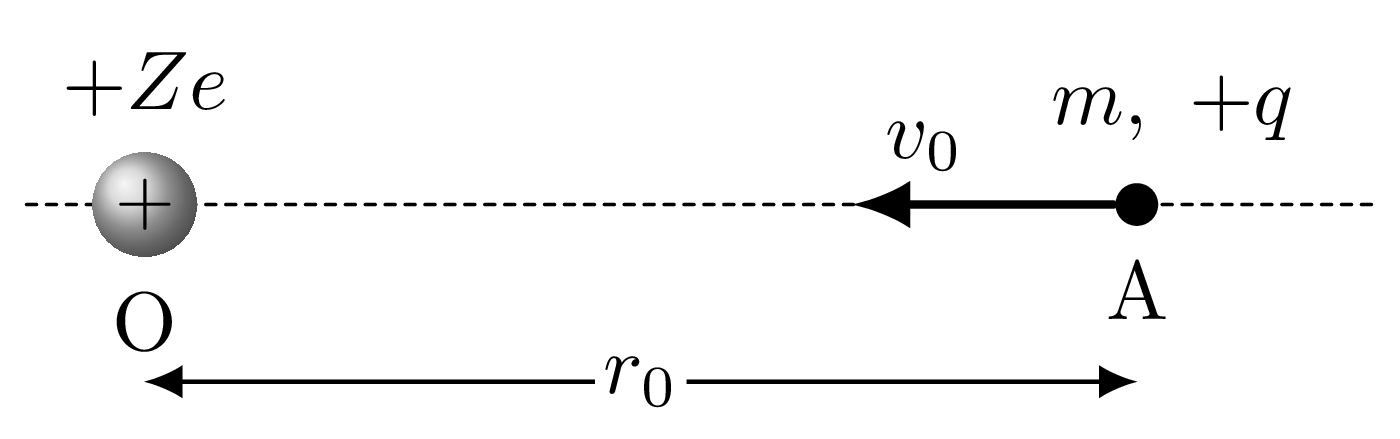
\includegraphics[keepaspectratio,width=66mm]{fig/n29_ex25_zu.png}\end{center}
\begin{komon}
\ko{1} 荷電粒子が距離$r\U{m}$のところまで接近してきたときの粒子の速さを$v\U{m/s}$とするとき，この点と点$\mathrm{A}$との間に成り立つ関係式をエネルギーの保存則より示せ．
\ko{2} 粒子は$\mathrm{O}$点からどれだけの距離まで近づくか．最接近距離を求めよ．
\ko{3} 粒子は最接近したのち，$\mathrm{O}$点から遠ざかっていく．遠ざかっていったときの最大の速さはいくらか．
\end{komon}
\end{reidai}

\begin{sisinE}
点電荷$+Ze$が距離$r$の点につくる電位は$k\dfrac{Ze}{r}$なので，粒子の位置エネルギーは$k\dfrac{Zeq}{r}$である．
最接近の瞬間は粒子が一瞬止まる（$v=0$）．
遠ざかるときは位置エネルギーが運動エネルギーに変わり続けるので，無限遠（位置エネルギー$0$）で速さが最大になる．
\end{sisinE}

\Key{点電荷$Q$から距離$r$の点の電位$V=k\dfrac{Q}{r}$（無限遠が基準）\quad $\dfrac{1}{2}mv^2+qV=$一定}

\begin{kaitou}
\begin{komon}
\ko{1} \Ana{\frac{1}{2}mv_0^2+k\frac{Zeq}{r_0}=\frac{1}{2}mv^2+k\frac{Zeq}{r}\Ans}
\ko{2} 最接近距離$r_{\min}$では$v=0$なので，(1)より
       \[\frac{1}{2}mv_0^2+k\frac{Zeq}{r_0}=k\frac{Zeq}{r_{\min}}\qquad\therefore\ r_{\min}=\frac{2kZeqr_0}{2kZeq+mv_0^2r_0}\U{m}\Ans\]
\ko{3} 無限遠で位置エネルギーが$0$になり，速さが最大$v_{\max}$となる：
       \[\frac{1}{2}mv_0^2+k\frac{Zeq}{r_0}=\frac{1}{2}mv_{\max}^2\qquad\therefore\ v_{\max}=\sqrt{v_0^2+\frac{2kZeq}{mr_0}}\U{m/s}\Ans\]
\end{komon}
\end{kaitou}
\end{reidaiunit}

\subsection{一様電場中の運動（電場偏向）}

一様な電場$E$の中で，電荷$q$の粒子は一定の力$qE$を受けるので，{\gtfamily 等加速度運動}をする．
電場に垂直に入射した粒子は，電場に垂直な方向には等速，電場の方向には等加速度で運動するので，{\gtfamily 放物線}を描く．
重力のかわりに$qE$がはたらく放物運動と考えればよい（負電荷は電場と逆向きに力を受ける）．
このように電場によって荷電粒子の進路を曲げることを{\gtfamily 電場偏向}という．

電子の電荷と質量の比$\dfrac{e}{m}$を{\gtfamily 比電荷}という．電子は非常に小さいので$e$や$m$を直接測ることは難しいが，電場や磁場による曲がり方は$\dfrac{e}{m}$だけで決まるので，比電荷は測定できる．19世紀の末にトムソンはこの方法で電子の比電荷を測定した（例題26）．現在知られている値は$\dfrac{e}{m}\fallingdotseq 1.76\times 10^{11}\U{C/kg}$である．

%%%%%%%%%%  例題26（原本の【例題30】）  %%%%%%%%%%%%%%%%%%%%
\bsNeed{70mm}
\begin{reidaiunit}
\begin{reidai}{トムソンの実験}
\hspace{1zw}真空中に図のような装置を置く．図の$x$軸の方向から電子が速さ$v_0\U{m/s}$でやってきて，金属板$\mathrm{A}$，$\mathrm{B}$の間（\MARU{1}の区間，長さ$l\U{m}$）を通過していく．金属板$\mathrm{A}$，$\mathrm{B}$にはそれぞれ電荷が蓄えられており，$\mathrm{AB}$間には上向き（$+y$の向き）に強さ$E\U{N/C}$の一様な電場が生じている．\MARU{1}の区間を通過した電子はその運動方向をねじ曲げられた後，\MARU{2}の区間を通過して距離$L\U{m}$だけ先にあるスクリーン上に到達する．この電子の運動に関して以下の問いに答えよ．ただし，重力の影響は無視してよいものとし，電子の電荷を$-e\U{C}$，電子の質量を$m\U{kg}$とする．
\begin{center}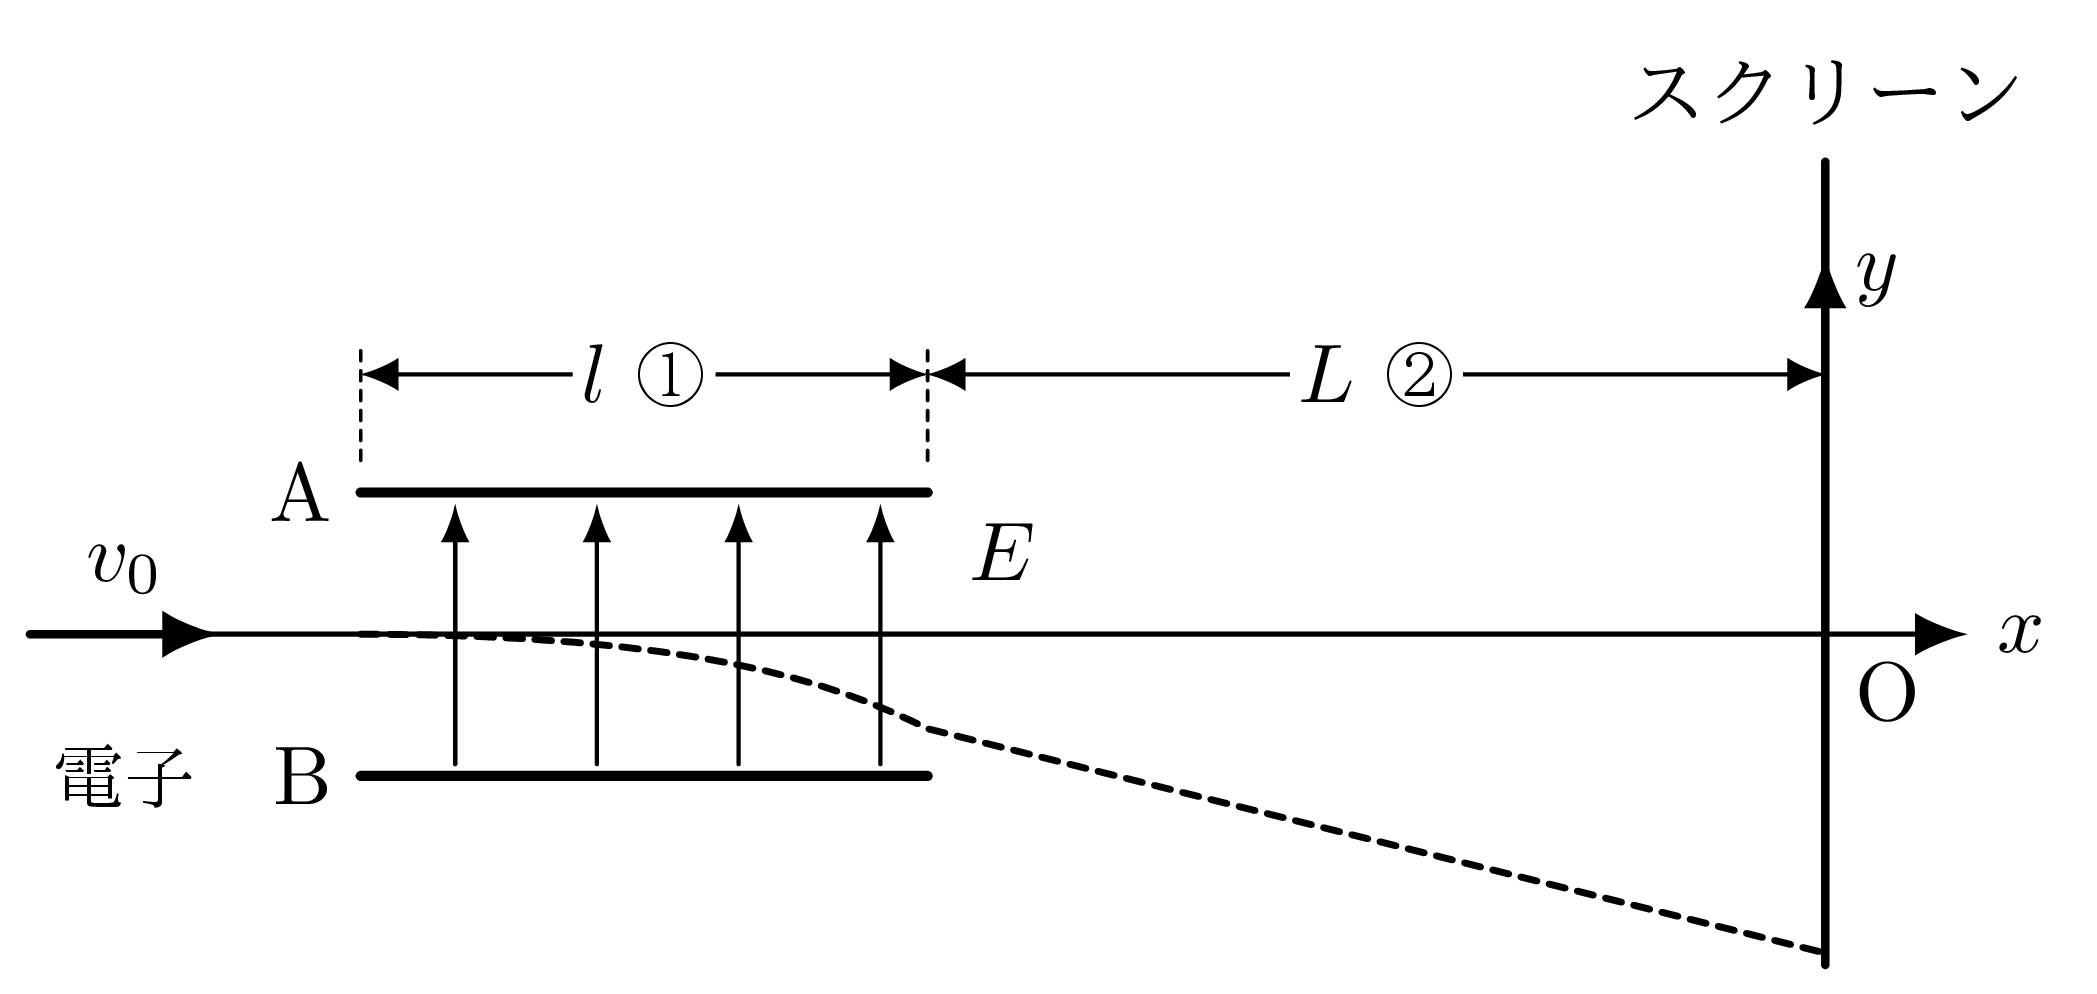
\includegraphics[keepaspectratio,width=100mm]{fig/n29_ex26_zu.png}\end{center}
\begin{komon}
\ko{1} 電子は\MARU{1}\MARU{2}の区間でそれぞれどのような運動をするか．
\ko{2} \MARU{1}の区間を通過し終える瞬間の，電子の速度$(v_x,v_y)\U{m/s}$を求めよ．
\ko{3} 電子が到達するスクリーン上の$y$座標$y\U{m}$を求めよ．
\ko{4} 電子の比電荷$\dfrac{e}{m}$を$y$などを利用して表せ．
\end{komon}
\end{reidai}

\begin{sisinE}
電子は負電荷なので，電場と逆向き（$-y$の向き）に$eE$の力を受ける．
\MARU{1}では$x$方向に等速，$y$方向に等加速度の放物運動，\MARU{2}では力を受けないので等速直線運動である．
\MARU{1}を通過する時間は$\dfrac{l}{v_0}$である．
\end{sisinE}

\Key{荷電粒子が電場から受ける力$qE$（負電荷は電場と逆向き）\quad 電場に垂直に入射すると放物運動}

\begin{kaitou}
\begin{komon}
\ko{1} \MARU{1}：{\gtfamily 放物運動}（$x$方向に等速，$-y$方向に等加速度）．\MARU{2}：{\gtfamily 等速直線運動}．\Ans
\ko{2} $y$方向の加速度は$-\dfrac{eE}{m}$，\MARU{1}の通過時間は$t_1=\dfrac{l}{v_0}$なので
       \[(v_x,\ v_y)=\Bigl(v_0,\ -\frac{eEl}{mv_0}\Bigr)\Ans\]
\ko{3} \MARU{1}での$y$方向の変位は$-\dfrac{1}{2}\dfrac{eE}{m}t_1^2=-\dfrac{eEl^2}{2mv_0^2}$．\MARU{2}の通過時間は$\dfrac{L}{v_0}$で，その間に$v_y\dfrac{L}{v_0}=-\dfrac{eElL}{mv_0^2}$だけ変位する．合わせて
       \Ana{y=-\frac{eEl}{mv_0^2}\Bigl(\frac{l}{2}+L\Bigr)\U{m}\Ans}
\ko{4} (3)を解いて
       \[\frac{e}{m}=-\frac{v_0^2\,y}{El\bigl(\frac{l}{2}+L\bigr)}\U{C/kg}\Ans\]
       （$y<0$なので右辺は正．$v_0$，$E$，$l$，$L$と$y$を測れば比電荷が求まる．）
       \begin{chuu}
       \MARU{2}での直線を後ろに延ばすと，\MARU{1}の区間のちょうど中央（入口から$\dfrac{l}{2}$）を通る．(3)の$\dfrac{l}{2}+L$はこのことを表している．
       \end{chuu}
\end{komon}
\end{kaitou}
\end{reidaiunit}

\subsection{ローレンツ力}

電流の流れている導線が磁場から力を受けるのは，電流の担い手として導線の中を{\gtfamily 移動している電子が磁場から力を受ける}からである．
磁場中を運動する荷電粒子が磁場から受ける力を{\gtfamily ローレンツ力}という．

\begin{zuright}{46mm}
\hspace{1zw}電気量の大きさが$q\U{C}$の荷電粒子が，磁束密度$B\U{T}$の{\gtfamily 磁場に垂直な速度成分}$v\U{m/s}$をもつとき，この粒子は大きさ
\AnaBD{f=qvB\U{N}}
のローレンツ力を受ける（磁場と角$\theta$をなす速度なら$f=qvB\sin\theta$）．
向きは，{\gtfamily 電荷の運動を電流に置き換えてフレミングの左手の法則}で決める．正電荷なら運動の向きが電流の向き，負電荷なら運動と逆向きが電流の向きである．
\zusep

\includegraphics[keepaspectratio,width=44mm]{text2_p66_fig1.png}
\end{zuright}

% 加筆：電磁力との関係（$F=IBl$ から $qvB$ が出ること）．
長さ$l$の導線内に速さ$v$で動く電荷$q$の粒子が$N$個あれば，電流は$I=\dfrac{Nqv}{l}$なので，電磁力$IBl=NqvB$は1個あたり$qvB$となり，ローレンツ力と一致する．

ローレンツ力は常に速度に垂直にはたらくので，{\gtfamily 仕事をしない}．
したがって，{\gtfamily 磁場は荷電粒子の速さを変えず，向きだけを変える}（この点が電場と大きく違う）．
一様な磁場に垂直な面内では，大きさ一定の力$qvB$が常に速度に垂直にはたらくので，粒子は{\gtfamily 等速円運動}をする．
円運動の運動方程式$m\dfrac{v^2}{r}=qvB$より，半径と周期は
\[r=\frac{mv}{qB},\qquad T=\frac{2\pi r}{v}=\frac{2\pi m}{qB}\]
であり，{\gtfamily 周期は速さによらない}（速い粒子ほど大きな円を描くが，一周にかかる時間は同じ）．

\bsNeed{44mm}
\begin{matome}{一様磁場中の荷電粒子の運動}
 \hspace{3mm} ローレンツ力：大きさ$qvB$（$v$は磁場に垂直な速度成分），向きは電流に置き換えてフレミングの左手の法則\\
 \MARU{1}\ 磁場に垂直な速度成分 → 磁場に垂直な面内で\AnaB{等速円運動}\qquad $r=\dfrac{mv}{qB}$，$T=\dfrac{2\pi m}{qB}$\\
 \MARU{2}\ 磁場に平行な速度成分 → ローレンツ力を受けないので\AnaB{一定}\\
 \hspace{3mm} 初速が磁場に平行なら等速直線運動，垂直なら等速円運動，斜めならら\,せん運動
\end{matome}

%%%%%%%%%%  例題27（原本の【例題28】）  %%%%%%%%%%%%%%%%%%%%
\bsNeed{60mm}
\begin{reidaiunit}
\begin{reidai}{磁場による荷電粒子の円運動}
\begin{zuright}{54mm}
\hspace{1zw}図の点線内には紙面に垂直で表から裏に向かう磁束密度$B\U{T}$の磁場がかけられている．スリット$\mathrm{S}_1$，$\mathrm{S}_2$を通った質量$m\U{kg}$，電荷の大きさ$q\U{C}$，速さ$v\U{m/s}$の粒子がこの磁場中で図のような半円を描いて磁場の外へ出た．このとき，以下の問いに答えよ．
\begin{komon}
\ko{1} 図から，この荷電粒子の電荷の符号を決定せよ．
\ko{2} 円運動の半径$R\U{m}$を求めよ．
\ko{3} 磁場中に入ってから半円を描いて出てくるまでに要する時間を求めよ．
\end{komon}
\zusep
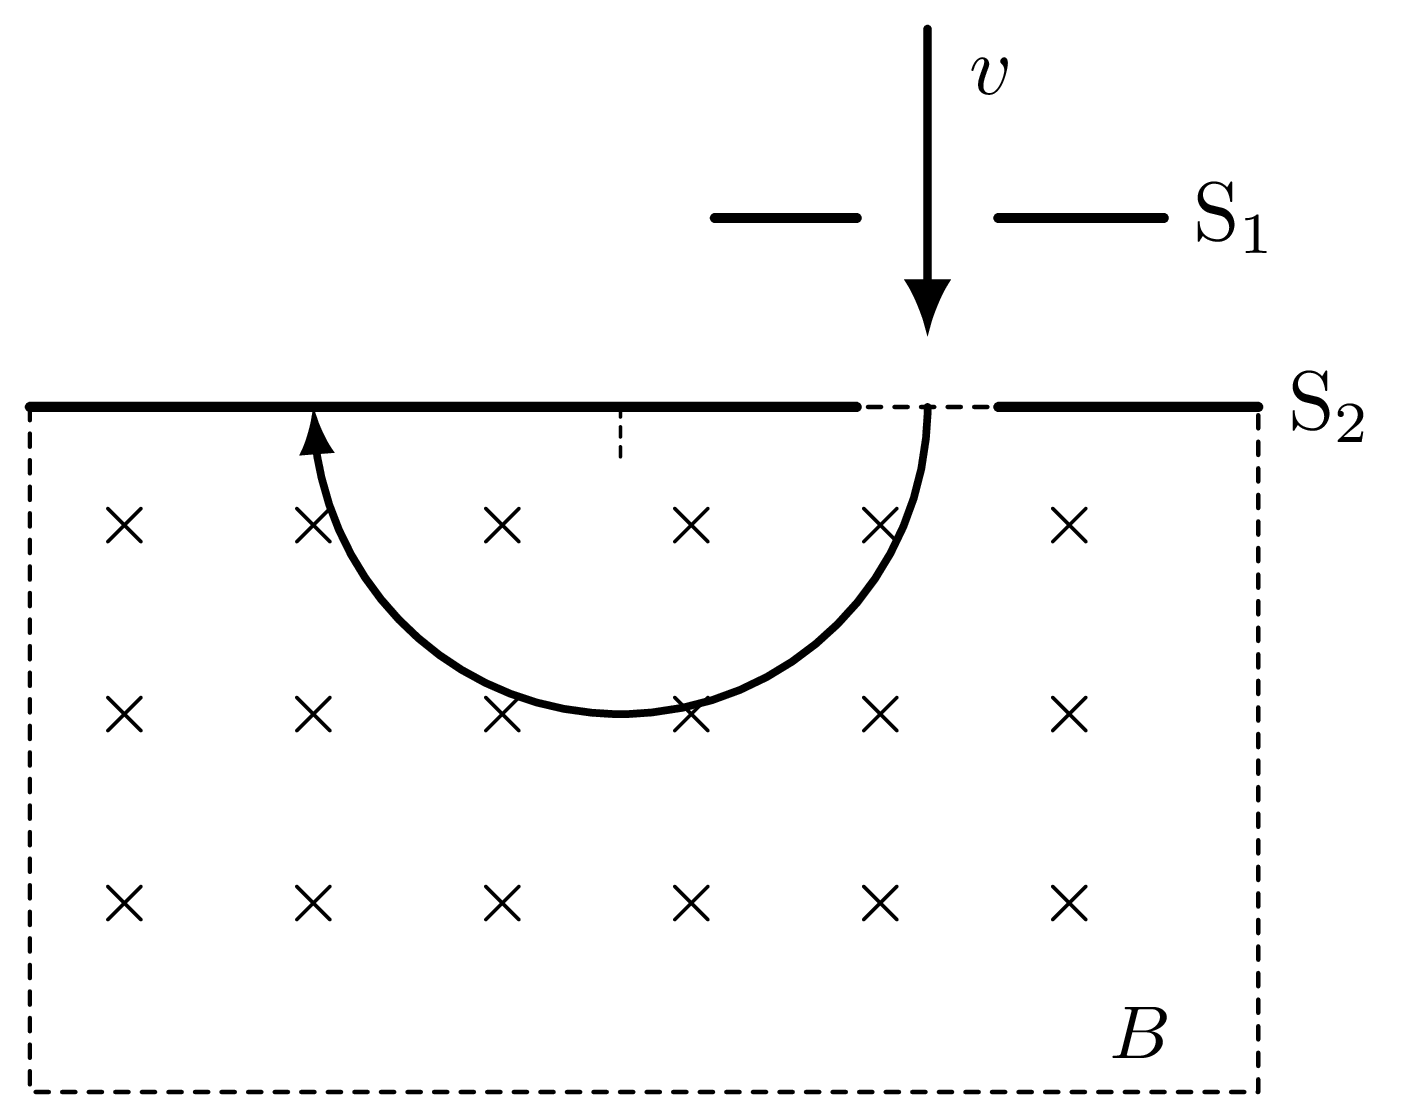
\includegraphics[keepaspectratio,width=50mm]{fig/n29_ex27_zu.png}
\end{zuright}
\end{reidai}

\begin{sisinE}
円運動の中心は，入射した点から見て図の左側にある．つまり入射した瞬間のローレンツ力は{\gtfamily 左向き}である．
正電荷と仮定してフレミングの左手の法則で力の向きを出し，それと比べる．
半径は半径方向（中心向き）の運動方程式から求める．
\end{sisinE}

\Key{ローレンツ力$qvB$，向きは電流に置き換えてフレミングの左手の法則\quad 円運動の運動方程式$m\dfrac{v^2}{r}=qvB$}

\begin{kaitou}
\begin{komon}
\ko{1} 正電荷なら，下向きの運動＝下向きの電流，磁場は紙面の奥向きなので，フレミングの左手の法則より力は{\gtfamily 右向き}になる．実際には左向きに曲がっているので，電荷は{\gtfamily 負}である．\Ans
\ko{2} 中心向きの運動方程式$m\dfrac{v^2}{R}=qvB$より
       \Ana{R=\frac{mv}{qB}\U{m}\Ans}
\ko{3} 半周なので
       \[t=\frac{\pi R}{v}=\frac{\pi m}{qB}\U{s}\Ans\]
\end{komon}
\end{kaitou}
\end{reidaiunit}

%%%%%%%%%%  例題28（原本の【例題29】）  %%%%%%%%%%%%%%%%%%%%
\bsNeed{70mm}
\begin{reidaiunit}
\begin{reidai}{磁場中における荷電粒子のらせん運動}
\begin{zuright}{44mm}
\hspace{1zw}$z$軸の正の向きに磁束密度の大きさ$B\U{T}$の一様な磁場がある．この磁場中に，質量$m\U{kg}$，正電荷$q\U{C}$をもつ粒子が，原点$\mathrm{O}$から$yz$平面内で$z$軸の正の向きと角度$\theta$をなす向き（$y$成分が正）に速さ$v\U{m/s}$で入射した．この粒子の運動を，$z$軸方向の運動と$xy$面内における運動とに分けて考えるとき，次の問いに答えよ．
\zusep
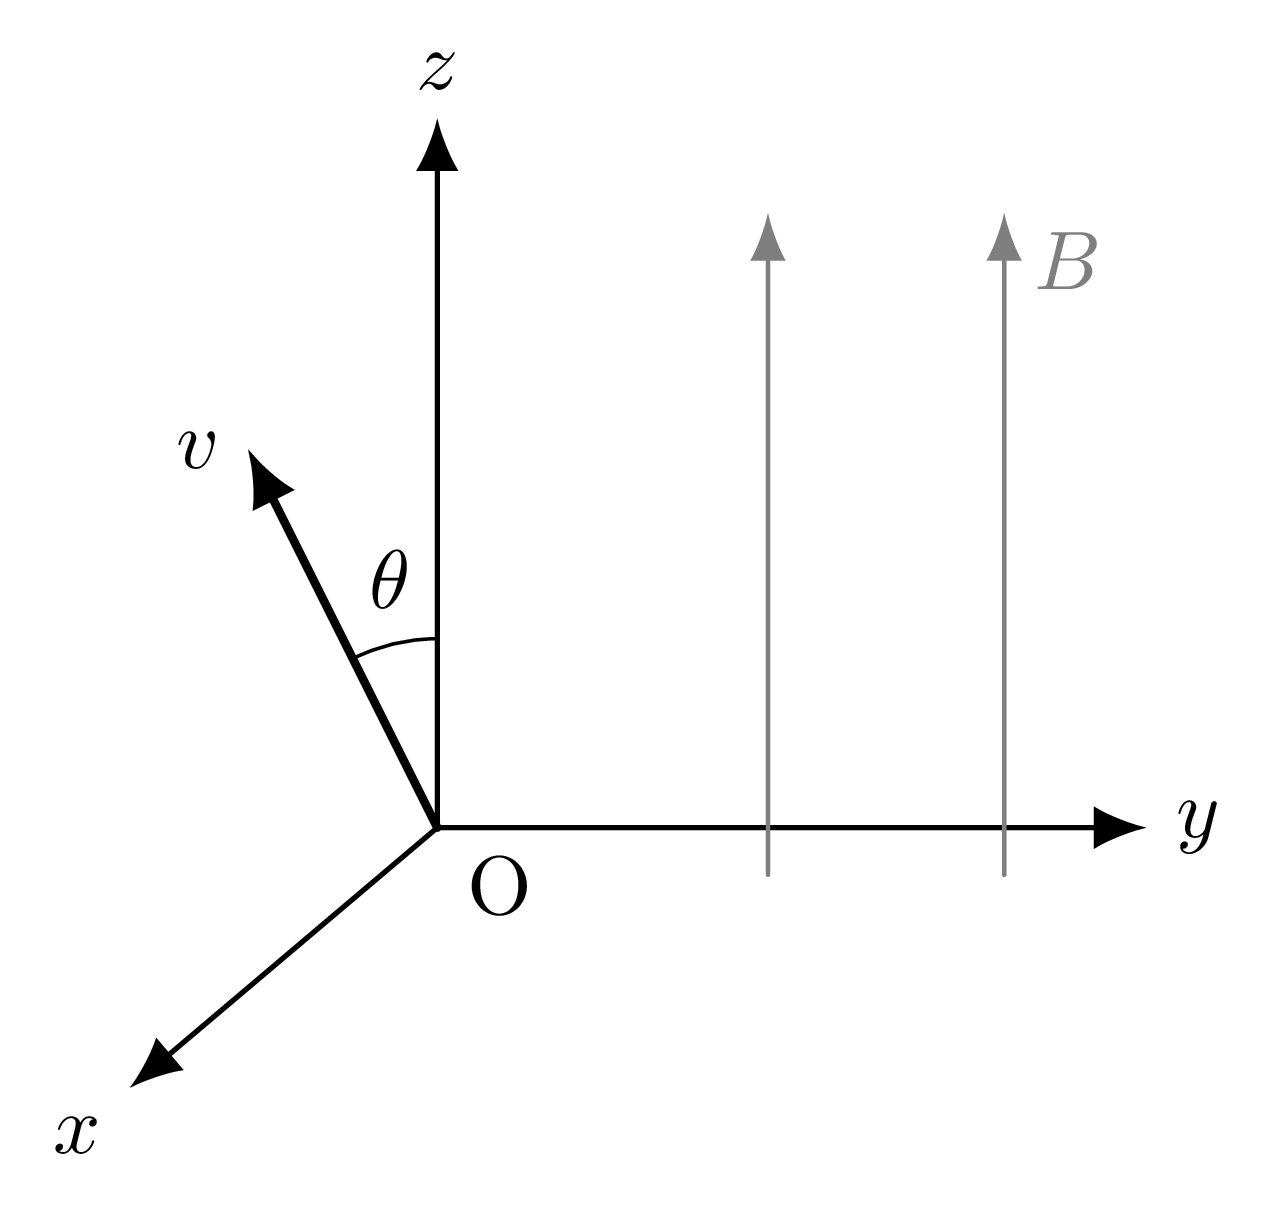
\includegraphics[keepaspectratio,width=40mm]{fig/n29_ex28_zu.png}
\end{zuright}
\hspace{1zw}まず，$xy$面内の運動について考える．
\begin{komon}
\ko{1} この粒子が点$\mathrm{O}$において受けるローレンツ力の向きと大きさを求めよ．
\ko{2} この粒子は$xy$面内では等速円運動を行う．この円運動の半径と周期，およびその中心の座標を求めよ．
\end{komon}
\hspace{1zw}次に，$z$軸方向の運動について考える．
\begin{komon}
\ko{3} $z$軸方向の運動はどのようなものか．説明せよ．
\ko{4} 以上の結果より，この粒子の運動を簡単に図示し，$z$軸方向のピッチ（1周する間に$z$方向に進む距離）を求めよ．
\end{komon}
\end{reidai}

\begin{sisinE}
速度を磁場に平行な成分$v\cos\theta$と垂直な成分$v\sin\theta$に分解する．
ローレンツ力は垂直な成分に対してだけはたらき，大きさは$q(v\sin\theta)B$である．
\end{sisinE}

\Key{速度を磁場に平行な成分と垂直な成分に分解する\quad 垂直な成分に対して円運動の運動方程式}

\begin{kaitou}
\begin{komon}
\ko{1} 磁場に垂直な速度成分は$+y$の向きに$v\sin\theta$．電流を$+y$，磁場を$+z$としてフレミングの左手の法則を使うと，力は{\gtfamily $+x$の向き}で，大きさは
       \[f=qvB\sin\theta\U{N}\Ans\]
\ko{2} $xy$面内の運動方程式$m\dfrac{(v\sin\theta)^2}{r}=q(v\sin\theta)B$より
       \Ana{r=\frac{mv\sin\theta}{qB}\U{m},\qquad T=\frac{2\pi r}{v\sin\theta}=\frac{2\pi m}{qB}\U{s}\Ans}
       原点で$+x$の向きに力を受けるので，中心は原点から$+x$の向きに$r$の点：
       \[\Bigl(\frac{mv\sin\theta}{qB},\ 0\Bigr)\Ans\]
\ko{3} $z$方向には力がはたらかないので，速さ$v\cos\theta$の{\gtfamily 等速直線運動}である．\Ans
\ko{4} $xy$面内の円運動と$z$方向の等速運動を合わせると，$z$軸に平行な軸のまわりの{\gtfamily らせん運動}になる．1周の間に$z$方向に進む距離（ピッチ）は
       \[v\cos\theta\cdot T=\frac{2\pi mv\cos\theta}{qB}\U{m}\Ans\]
\end{komon}
\end{kaitou}
\end{reidaiunit}

\subsection{磁場偏向と比電荷}

トムソンの実験（例題26）では電場によって電子の進路を曲げた（電場偏向）．
これに対して，荷電粒子が磁場中で円軌道を描くことを利用して進路を曲げる方法もあり，これを{\gtfamily 磁場偏向}という．
円の半径$r=\dfrac{mv}{qB}$も$\dfrac{q}{m}$（比電荷）だけで決まるので，磁場偏向からも比電荷を求めることができる．

電場偏向と磁場偏向を比べると，次のような違いがある．
\begin{description}
\item[\MARU{1}] 電場は粒子に仕事をするので{\gtfamily 速さが変わる}．磁場は仕事をしないので{\gtfamily 速さは変わらない}．
\item[\MARU{2}] 一様な電場中の軌道は{\gtfamily 放物線}，一様な磁場中の軌道は{\gtfamily 円（の一部）}である．
\end{description}

%%%%%%%%%%  例題29（原本の【例題31】）  %%%%%%%%%%%%%%%%%%%%
\bsNeed{60mm}
\begin{reidaiunit}
\begin{reidai}{磁場偏向}
\hspace{1zw}真空中に図のような装置を置く．図の$x$軸の方向から電子が速さ$v\U{m/s}$でやってきて，紙面の奥から手前に向かう一様な磁束密度$B\U{T}$の磁場がかかった\MARU{1}の区間（長さ$l\U{m}$）を通過していく．\MARU{1}の区間を通過した電子はその運動方向をねじ曲げられた後，\MARU{2}の区間を通過して距離$L\U{m}$だけ先にあるスクリーン上に到達する．この電子の運動に関して以下の問いに答えよ．ただし，重力の影響は無視してよいものとし，電子の電荷を$-e\U{C}$，電子の質量を$m\U{kg}$とする．
\begin{center}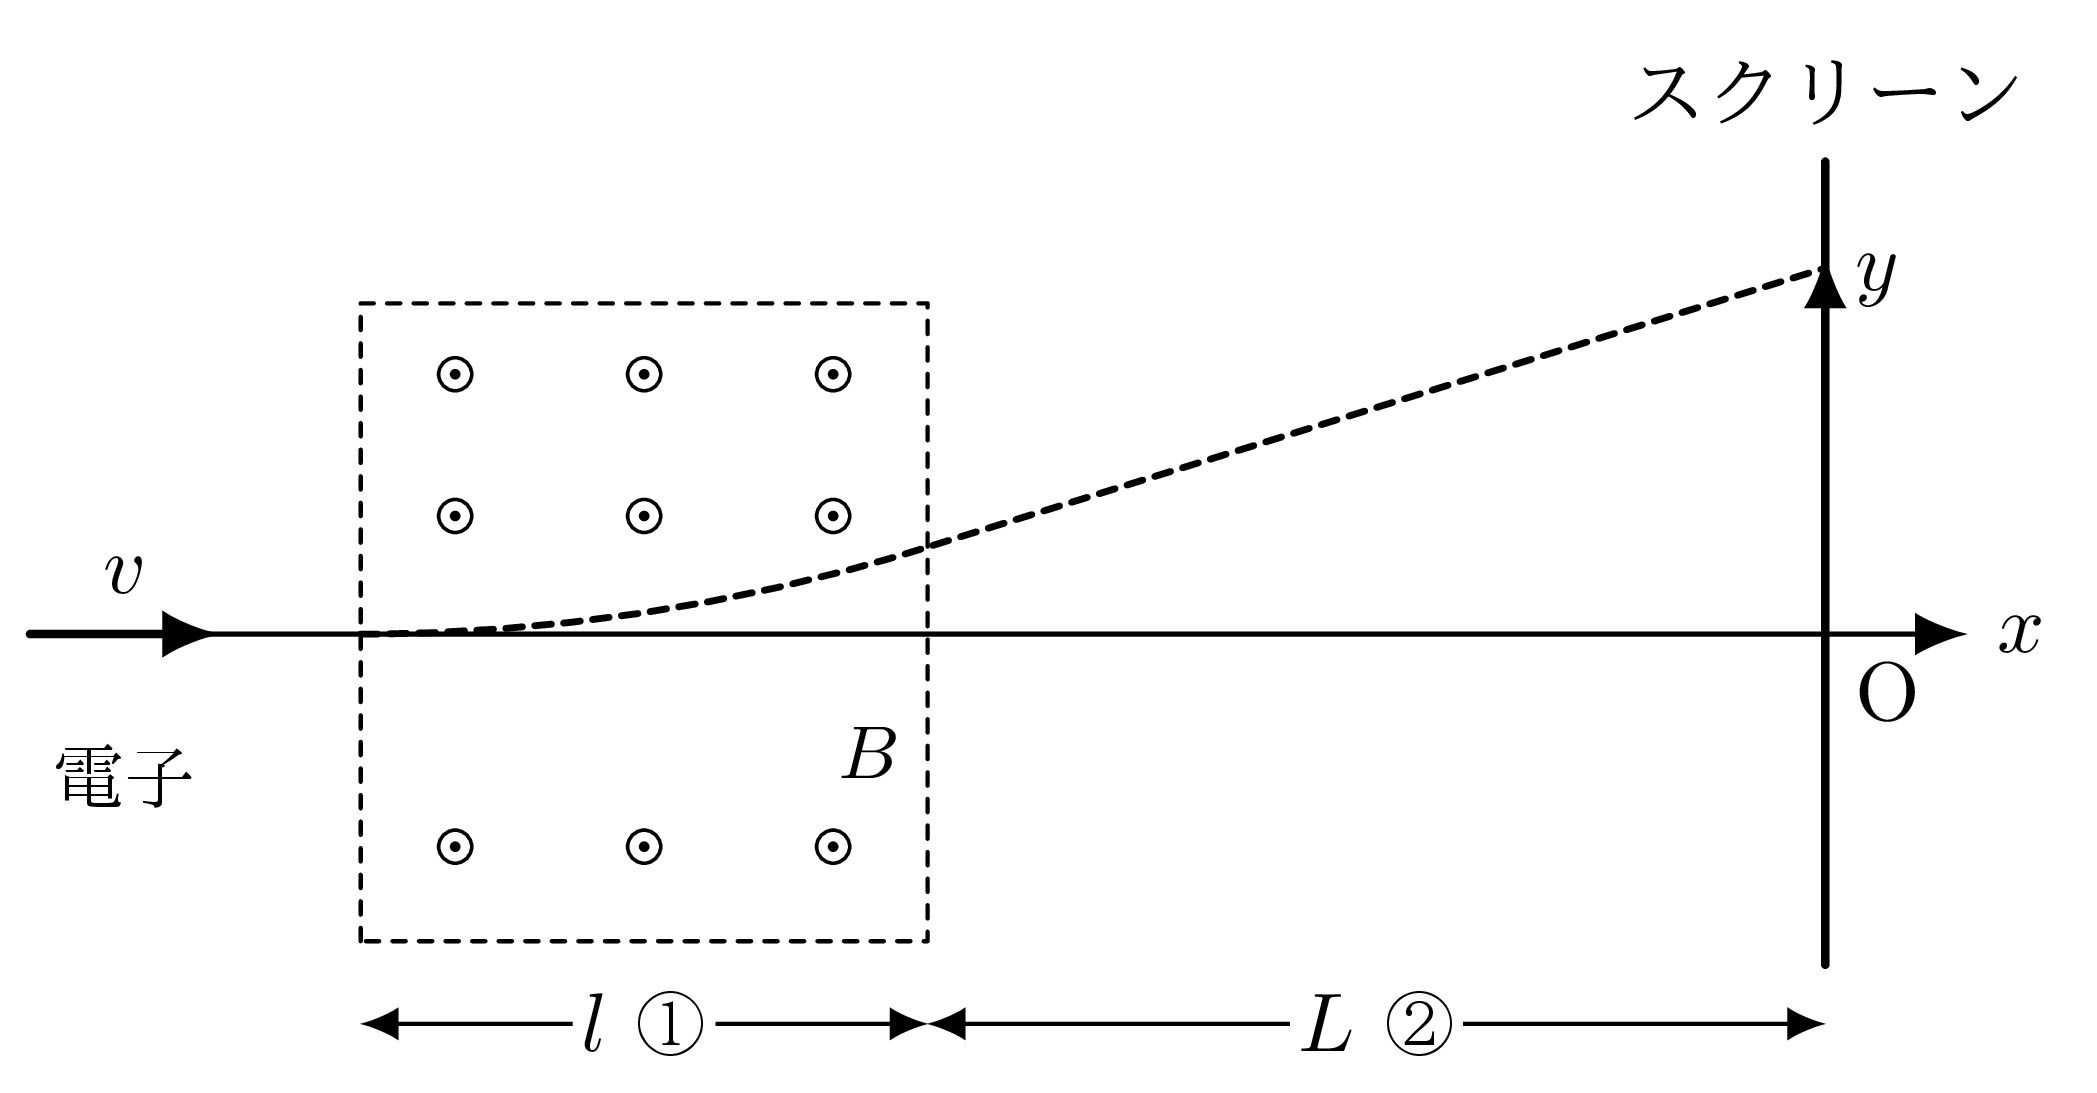
\includegraphics[keepaspectratio,width=100mm]{fig/n29_ex29_zu.png}\end{center}
\begin{komon}
\ko{1} \MARU{1}の区間では電子は円運動の一部を行う．この円運動の半径$r\U{m}$を求めよ．
\ko{2} $r$が$l$より十分大きいとして，電子が到達するスクリーン上の$y$座標$y\U{m}$を求めよ．
\ko{3} 電子の比電荷$\dfrac{e}{m}$を$y$などを利用して表せ．
\end{komon}
\end{reidai}

\begin{sisinE}
(2) $r\gg l$なら，\MARU{1}での曲がり角$\varphi$は小さく，$\varphi\fallingdotseq\dfrac{l}{r}$である（弧の長さ$\fallingdotseq l$）．\MARU{1}での$y$方向のずれは$\dfrac{l^2}{2r}$程度で，\MARU{2}では傾き$\varphi$の直線で進む．例題26と同じく，\MARU{2}の直線は\MARU{1}の中央を通ると考えてよい．
\end{sisinE}

\Key{ローレンツ力の向きは電流に置き換えてフレミングの左手の法則\quad $r=\dfrac{mv}{eB}$}

\begin{kaitou}
\begin{komon}
\ko{1} 運動方程式$m\dfrac{v^2}{r}=evB$より
       \[r=\frac{mv}{eB}\U{m}\Ans\]
\ko{2} 電子の運動と逆向き（$-x$）が電流の向き．磁場は手前向きなので，フレミングの左手の法則より力は$+y$の向きで，電子は$+y$側に曲がる．\MARU{1}での曲がり角は$\varphi\fallingdotseq\dfrac{l}{r}$，\MARU{1}でのずれは$\fallingdotseq\dfrac{l^2}{2r}$なので
       \Ana{y\fallingdotseq\frac{l^2}{2r}+L\frac{l}{r}=\frac{eBl}{mv}\Bigl(\frac{l}{2}+L\Bigr)\U{m}\Ans}
\ko{3} (2)より
       \[\frac{e}{m}=\frac{vy}{Bl\bigl(\frac{l}{2}+L\bigr)}\U{C/kg}\Ans\]
       \begin{chuu}
       電場偏向（例題26）では$y\propto\dfrac{1}{v^2}$，磁場偏向では$y\propto\dfrac{1}{v}$である．両方を測れば$v$を消去して比電荷が決まる．実際のトムソンの実験は，次の速度選別器の考え方で$v$を求めていた．
       \end{chuu}
\end{komon}
\end{kaitou}
\end{reidaiunit}

% 加筆：速度選別器・ホール効果・サイクロトロン（再編案「練習前にまとめる」．練習［95］［96］［98］）．
\subsection{電場と磁場を組み合わせた装置}

\begin{zuright}{34mm}
\noindent\MARU{1}\ {\gtfamily 速度選別器}

\hspace{1zw}右図のように，粒子の進む向きに垂直な電場$E$と，それらの両方に垂直な磁場$B$を同時にかける．正電荷$q$の粒子は電場から$qE$，磁場から逆向きに$qvB$の力を受ける．2つがつり合う
\[qE=qvB\qquad\text{すなわち}\qquad v=\frac{E}{B}\]
の速さの粒子だけが直進し，それ以外の粒子は曲げられてスリットを通れない．こうして特定の速さの粒子だけを取り出すことができる（練習［95］）．
\zusep
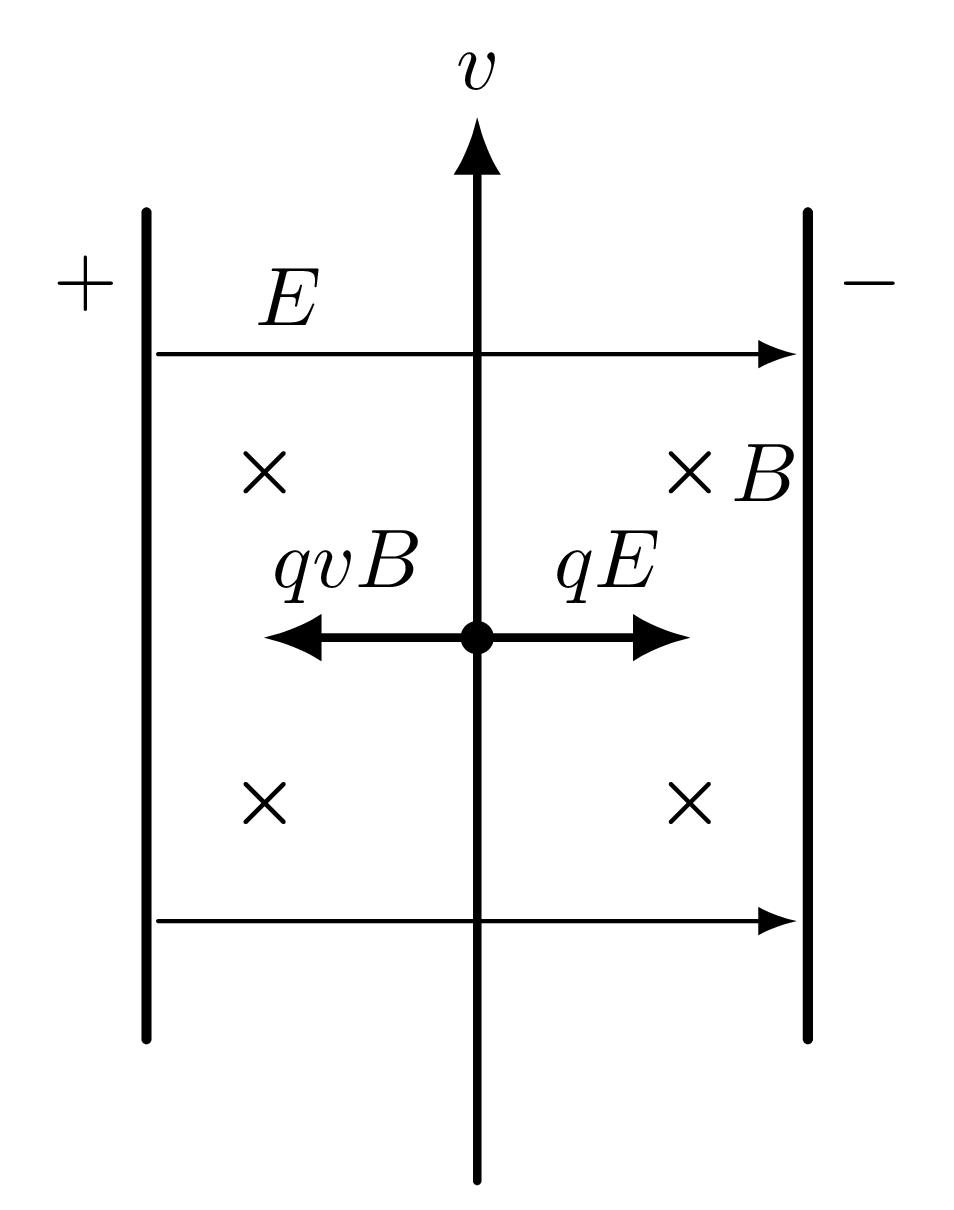
\includegraphics[keepaspectratio,width=32mm]{fig/n29_zu_sokudo.png}
\end{zuright}

\begin{zuright}{46mm}
\noindent\MARU{2}\ {\gtfamily ホール効果}

\hspace{1zw}電流の流れている導体（半導体）に，電流に垂直に磁場をかけると，キャリアがローレンツ力で曲げられて一方の面に集まり，向かい合う面の間に電位差（{\gtfamily ホール電圧}）が生じる．
集まった電荷の作る電場から受ける力がローレンツ力とつり合うと，それ以上は集まらなくなる．
キャリアが正（正孔）か負（電子）かでホール電圧の正負が逆になるので，半導体のキャリアの種類を判定できる（練習［96］）．
\zusep
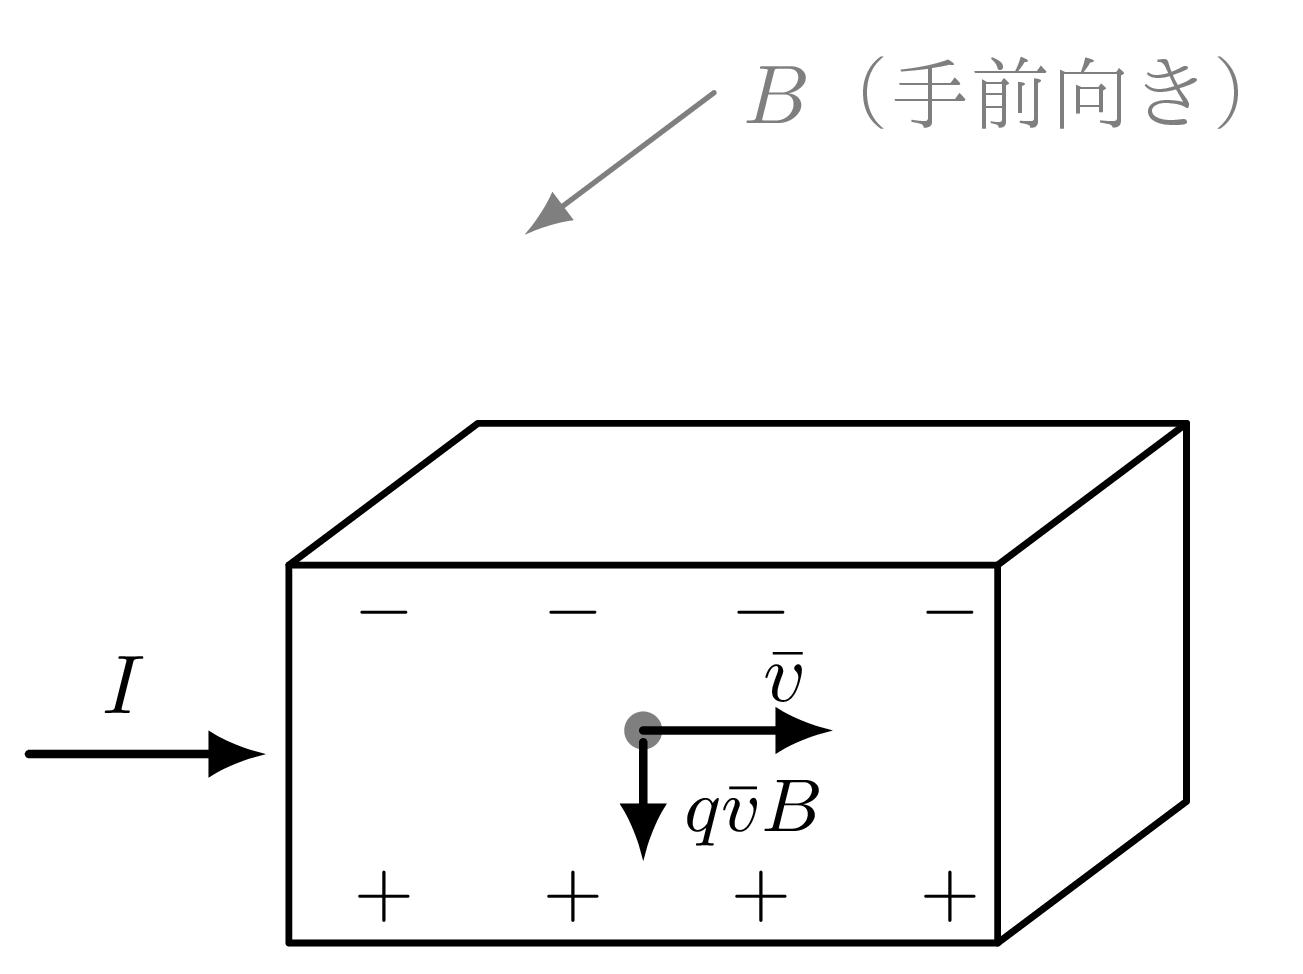
\includegraphics[keepaspectratio,width=44mm]{fig/n29_zu_hall.png}
\end{zuright}

\begin{zuright}{56mm}
\noindent\MARU{3}\ {\gtfamily サイクロトロン}

\hspace{1zw}磁場中に2つのD字形の中空電極を向かい合わせて置き，そのすき間に交流電圧をかける．粒子は電極の中では磁場によって半円を描き，すき間を通るたびに電場で加速される．
円運動の{\gtfamily 周期$T=\dfrac{2\pi m}{qB}$は速さによらない}ので，交流電圧の周期を$T$に合わせておけば，粒子は半周ごとに必ず加速され，半径を大きくしながら加速され続ける（練習［98］）．
\zusep
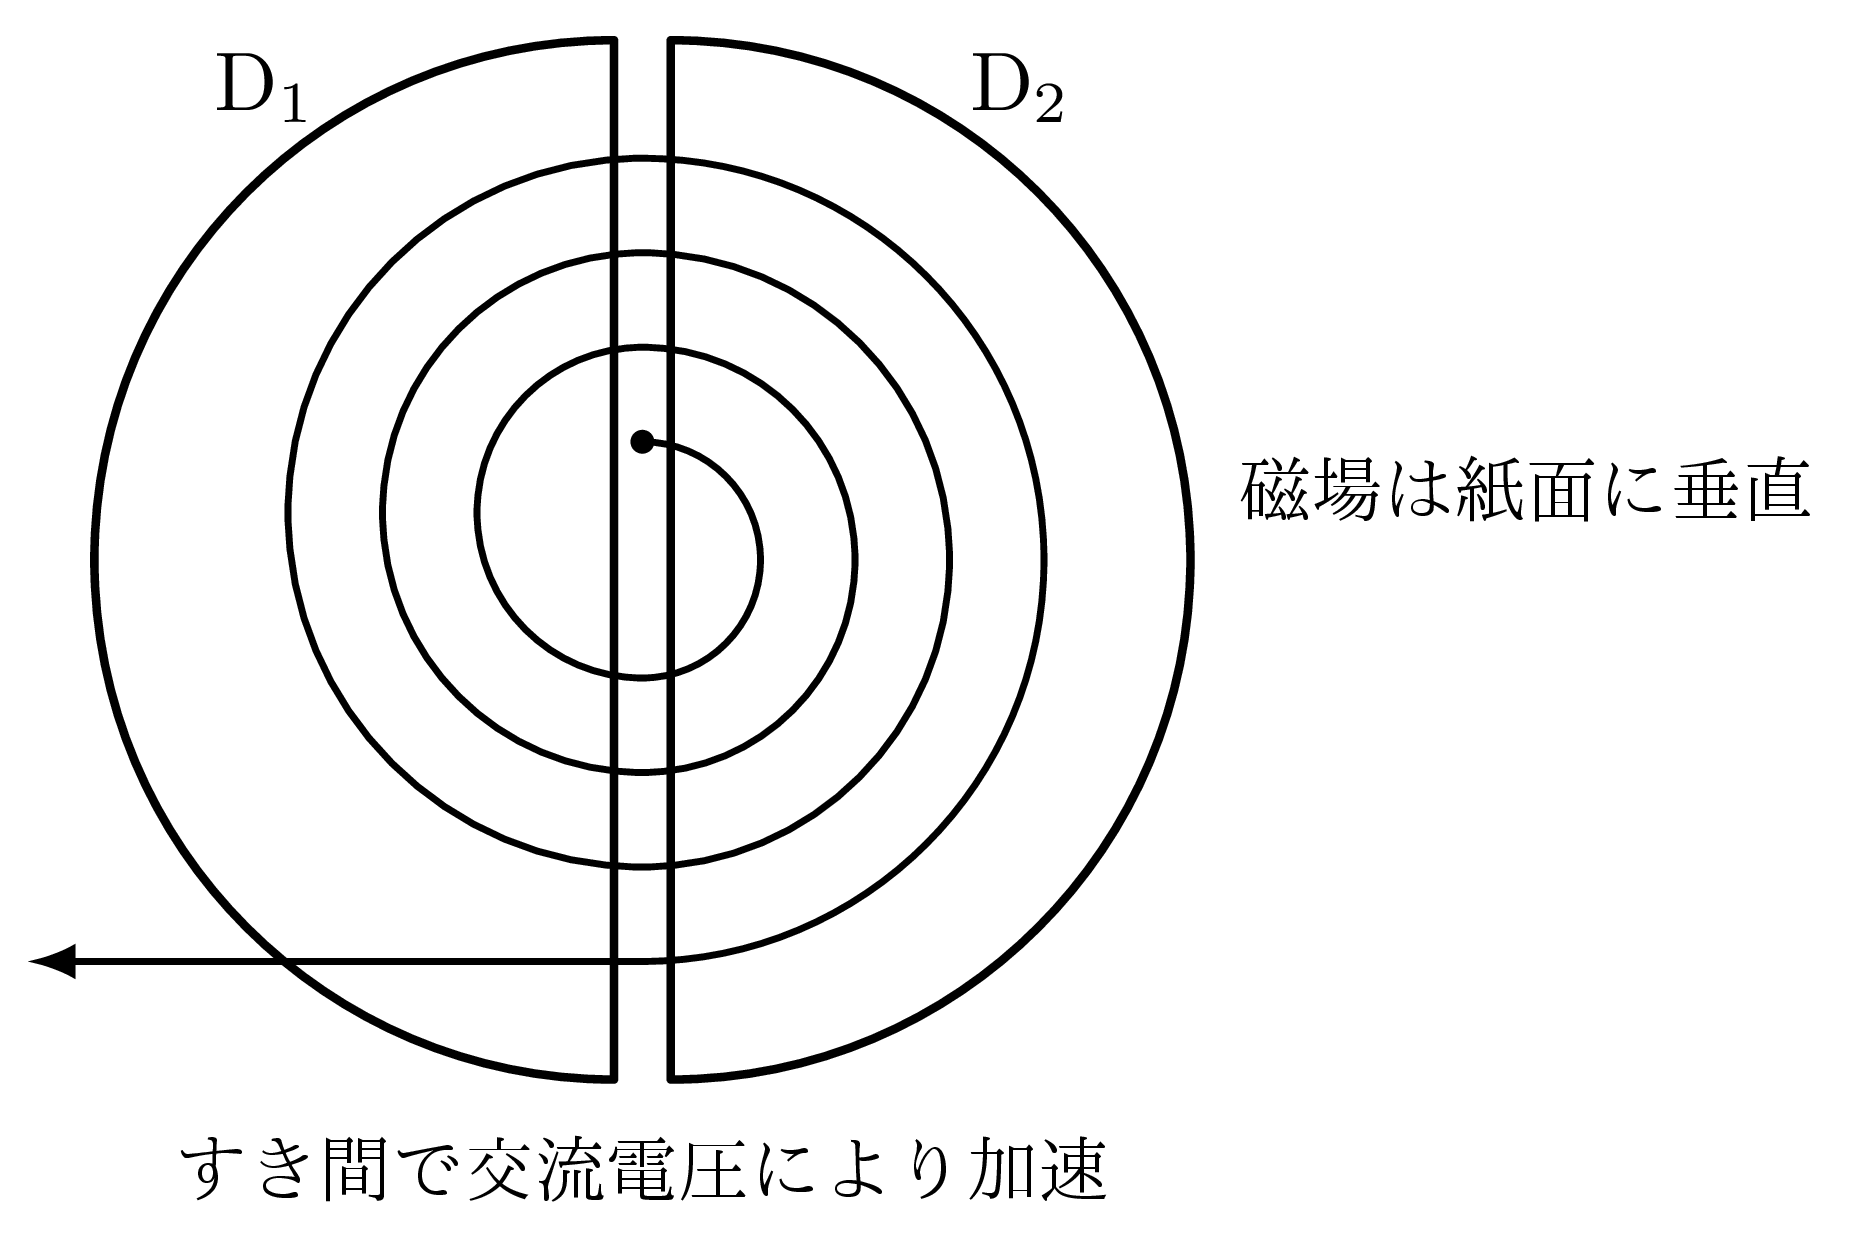
\includegraphics[keepaspectratio,width=54mm]{fig/n29_zu_cyclo.png}
\end{zuright}

\newpage

%%%%%%%%%%%%%%%%%%%%  練習問題  %%%%%%%%%%%%%%%%%%%%
% 第28回の［89］に続く．
\setcounter{qno}{89}

\filbreak
\Rank{A問題}

\Mon{基本公式の確認}

\hspace{1zw}以下の設問に答えよ．ただし真空の透磁率を$\mu_0=4\pi\times 10^{-7}\U{Wb/A\cdot m}$，電子の質量を$m_e=9.1\times 10^{-31}\U{kg}$，電荷を$-e=-1.6\times 10^{-19}\U{C}$とする．
\begin{komon}
\ko{1} 強さ$20\U{A/m}$の一様な磁場に対して垂直に長さ$0.10\U{m}$の導線を置き，強さ$2.0\U{A}$の電流を流した．導線が磁場から受ける力の大きさは何$\U{N}$か．
\ko{2} 磁束密度の大きさ$1.4\U{Wb/m^2}$の一様な磁場に対して垂直に速さ$1.6\times 10^7\U{m/s}$の電子を入射させたとき，電子の描く円運動の半径は何$\U{m}$か．また周期は何$\U{s}$か．
\end{komon}

\filbreak
\Rank{B問題}

\Mon{複数の点電荷による電位の合成}

\begin{zuright}{50mm}
\hspace{1zw}図に示すように，紙面上に$x$-$y$直交座標系を設定し，原点から距離$l\U{m}$だけ離れた$x$軸上の点$\mathrm{A}$に正の点電荷$+q\U{C}$を，点$\mathrm{B}$に負の点電荷$-q\U{C}$を固定した．原点$\mathrm{O}$から距離$d\U{m}$（ただし$d>l>0$とする）だけ離れた点をそれぞれ$\mathrm{P}$，$\mathrm{Q}$，$\mathrm{R}$とし，クーロンの法則の比例定数を$k\U{N\cdot m^2/C^2}$とする．以下の設問に答えよ．
\begin{komon}
\ko{1} 点$\mathrm{P}$，$\mathrm{Q}$，$\mathrm{R}$の電位$V_{\mathrm{P}}$，$V_{\mathrm{Q}}$，$V_{\mathrm{R}}$をそれぞれ求めよ．ただし，無限遠方を電位の基準点とする．
\end{komon}
\zusep
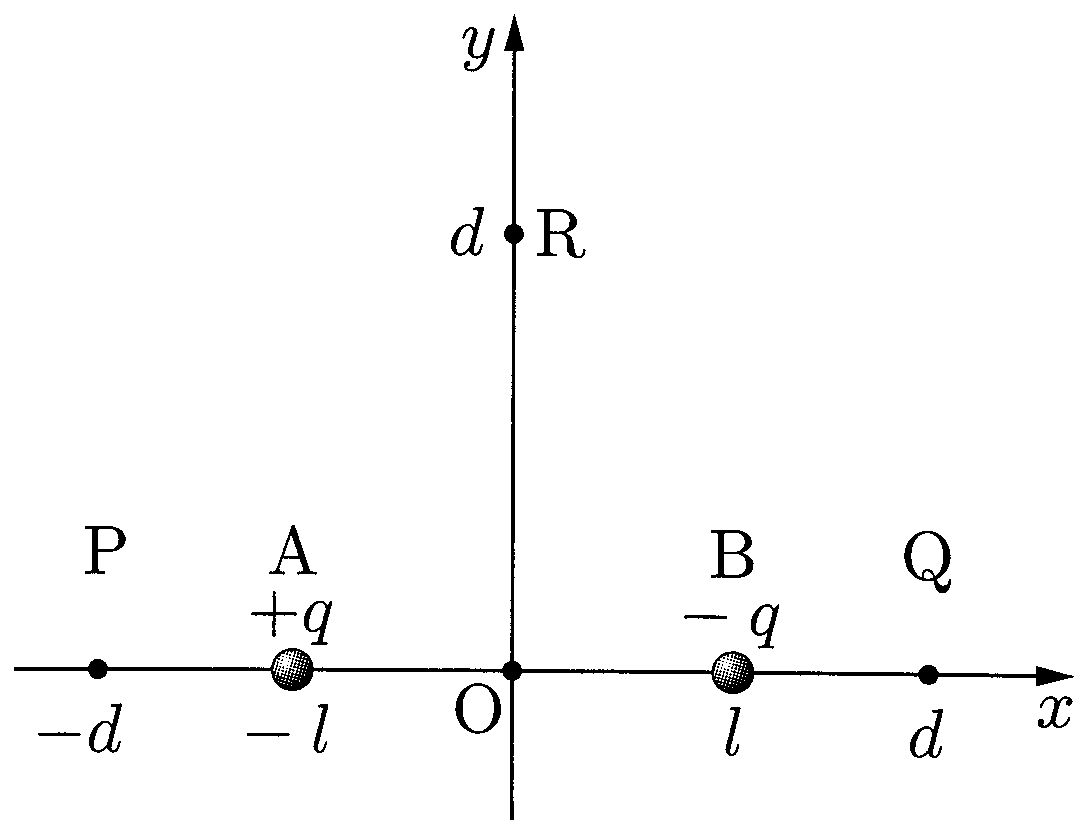
\includegraphics[keepaspectratio,width=48mm]{fig/n29_p90_zu.png}
\end{zuright}
\begin{komon}
\ko{2} 点$\mathrm{Q}$に正の電荷$+q\U{C}$を持った質量$m\U{kg}$の質点を置き，これに$+x$の方向に初速$v_0\U{m/s}$を与えた．このとき，この質点が無限遠方に飛び去るためには初速$v_0$がいくら以上でなければならないか．ただし，重力は無視してよい．
\end{komon}

\Mon[\Sitei]{磁場中の荷電粒子の運動}

\begin{zuright}{56mm}
\hspace{1zw}右図のように間隔$d\U{m}$で平行に置かれた2枚の平行極板があり，極板間には磁束密度$B\U{Wb/m^2}$の一様な磁場が紙面に対して垂直に裏→表向きにかかっている．図のように，質量$m\U{kg}$，電荷$q\U{C}$（$>0$）の正電荷を持つ荷電粒子が，一方の電極から極板に対して垂直に速さ$v\U{m/s}$で飛び出したとする．極板間には電場はなく，重力の影響は無視してよい．
\zusep
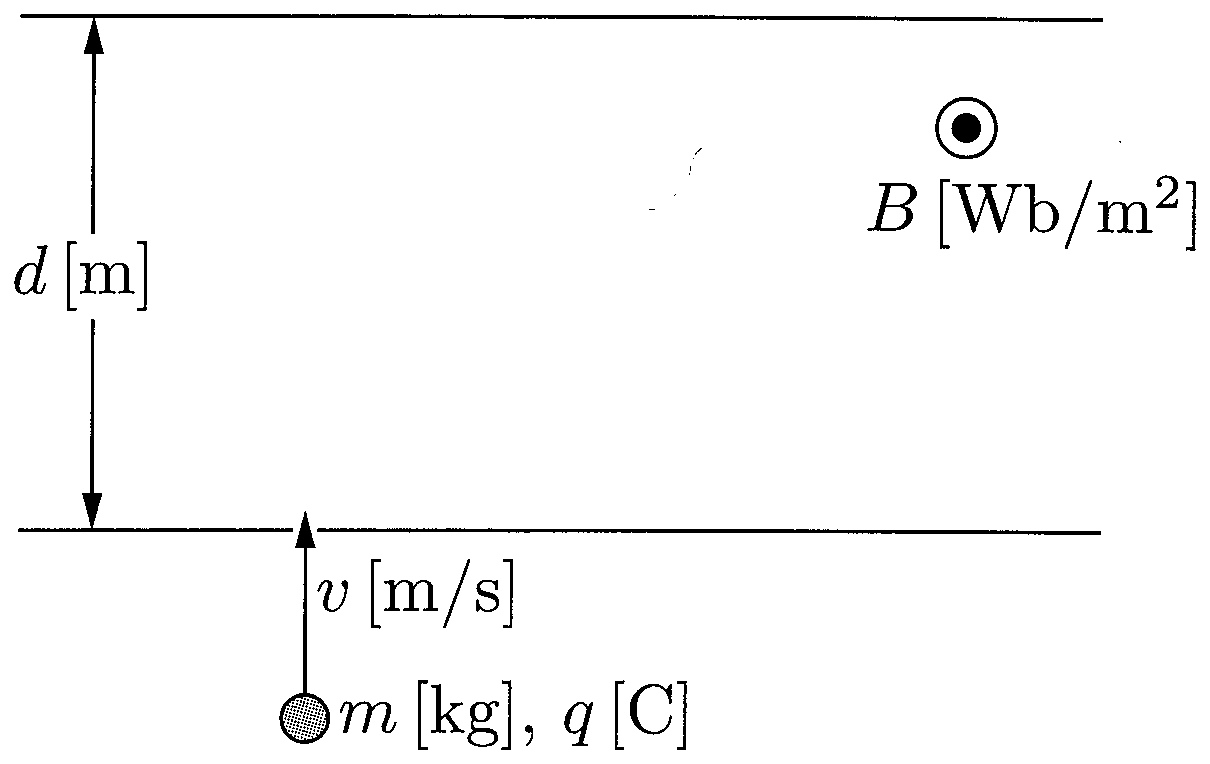
\includegraphics[keepaspectratio,width=54mm]{fig/n29_p92_zu.png}
\end{zuright}
\begin{komon}
\ko{1} この粒子が対極に到達しないための$d$についての条件を求めよ．
\ko{2} この粒子が対極に到達するような範囲で極板間隔$d\U{m}$を適当に変化させる．このとき，この粒子が極板を飛び出してから対極に到達するまでの時間が最大値になるのは$d$がいくらのときか．また，そのときの最大所要時間の値$t_{\max}\U{s}$を求めよ．
\end{komon}

\Mon{磁場中での電子のらせん運動}

\begin{zuright}{46mm}
\hspace{1zw}右図のように長さ$l\U{m}$の円筒に一様に$N$回巻いたコイルに，可変抵抗および電池を接続して強さ$I\U{A}$の電流を流したところ，コイルの内側には一様な磁場が生じた．この磁場中に速度ベクトルが$(0,\,v_\perp,\,v_{/\!/})\U{m/s}$と表される初速度を持つ電子を右図の原点$\mathrm{O}$に入射させたところ，この電子は磁場からローレンツ力を受けてコイル内をらせん運動をし，再び$z$軸上の点$\mathrm{S}$を通過した．電子の電荷を$-e\U{C}$，真空の透磁率を$\mu_0\U{Wb^2/N\cdot m^2}$として以下の問いに答えよ．
% 原本の透磁率の単位は Wb/N·m² （Wb² の誤植）．
\begin{komon}
\ko{1} コイル内部に生じる磁場の向きと強さ$H\U{A/m}$を求めよ．
\ko{2} らせん運動を$xy$平面に投影したときの中心の座標，およびこの粒子が$\mathrm{O}$点を出発してから$\mathrm{S}$点に到達するまでに要する時間を求めよ．
\ko{3} $\overline{\mathrm{OS}}$の長さを求めよ．
\end{komon}
\zusep
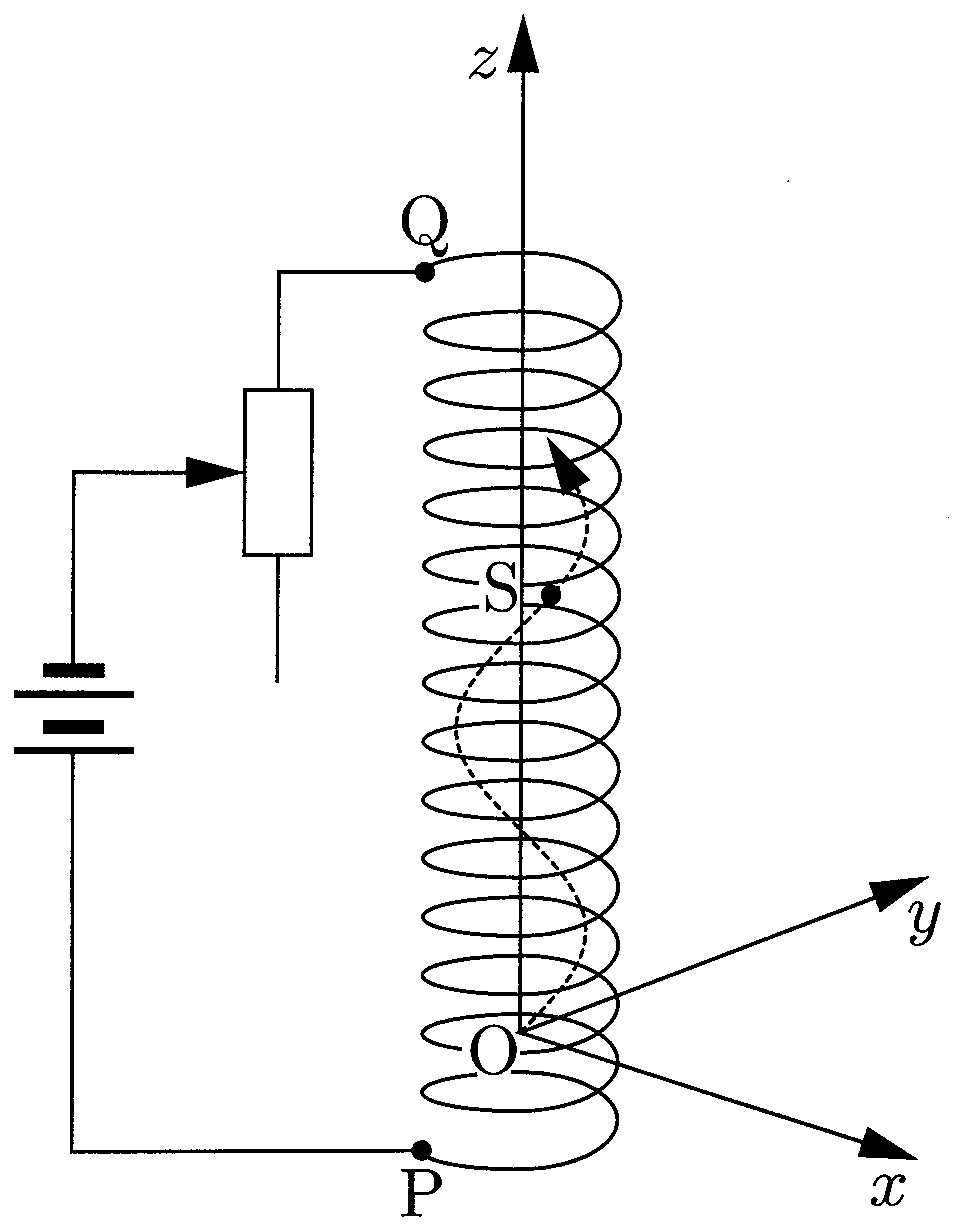
\includegraphics[keepaspectratio,width=42mm]{fig/n29_p93_zu.png}
\end{zuright}

\Mon[\Sitei]{トムソンの実験}

\hspace{1zw}図のような装置において電位$-V_0=-3.0\times 10^2\U{V}$の陰極$\mathrm{K}$から電子を初速$0$で放出すると，電子は細孔$\mathrm{H}$，$\mathrm{H}^\prime$を通り，電極板$\mathrm{D}$，$\mathrm{D}^\prime$に平行に入射し，蛍光面$\mathrm{G}$上の点$\mathrm{O}$に衝突する．$\mathrm{G}$にぶつかった電子は塗付されている蛍光材料により蛍光を発するため，このような装置を使うと電子線が電極板によりどの位置にねじ曲げられたかが分かる仕組みになっている．
\begin{center}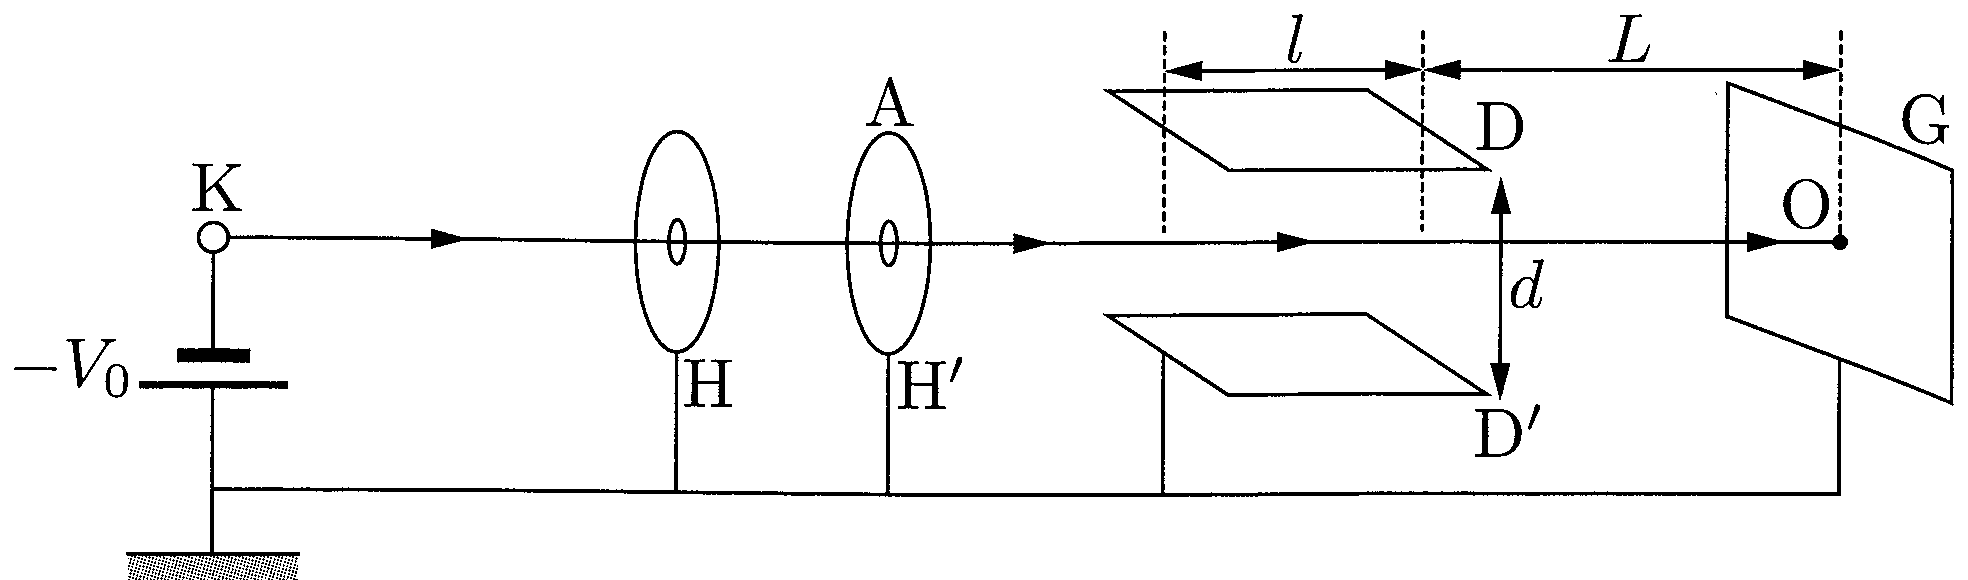
\includegraphics[keepaspectratio,width=110mm]{fig/n29_p94_zu.png}\end{center}
\hspace{1zw}今，陰極$\mathrm{K}$から電子を発生させ，細孔$\mathrm{H}$，$\mathrm{H}^\prime$を毎秒$1.0\times 10^9$個の電子が通過するようにした．$\mathrm{D}$，$\mathrm{D}^\prime$はそれぞれ一辺が$l=1.0\times 10^{-1}\U{m}$の正方形の導体平板で，間隔$d=1.0\times 10^{-2}\U{m}$，その端から蛍光面$\mathrm{G}$までの距離は$L=1.0\U{m}$になっている．$\mathrm{H}$，$\mathrm{H}^\prime$，$\mathrm{D}^\prime$，$\mathrm{G}$は接地されており，また装置全体は真空中にある．真空の誘電率$\varepsilon_0=8.9\times 10^{-12}\U{F/m}$，電子の質量$m=9.1\times 10^{-31}\U{kg}$，電荷$-e=-1.6\times 10^{-19}\U{C}$とし，$\mathrm{D}$，$\mathrm{D}^\prime$が作る電場は極板の端でも板に垂直であるとして，以下の設問に答えよ．重力の影響は無視してよい．
\begin{komon}
\ko{1} 力学的エネルギー保存則より，電子が細孔$\mathrm{H}$を通過するときの速さ$v_0$を求めよ．
\ko{2} 極板$\mathrm{D}$の電荷が$0$のときは，極板間に電場がないため，電子は次々と蛍光面$\mathrm{G}$上の点$\mathrm{O}$に衝突し，点$\mathrm{O}$に輝点を生じる．極板$\mathrm{D}$に電荷を与えると，極板間に生じる電場により電子の流れがねじ曲げられ，電子の衝突点は点$\mathrm{O}$からずれる．そのため，スクリーン上の輝点は点$\mathrm{O}$からずれる．ところが，極板$\mathrm{D}$に与える電荷$Q$（$>0$）がある値$Q_0$以上の場合には輝点が一瞬消え，短時間後にある定点$\mathrm{P}$（$Q$によらない）が光るようになる．電荷を与えてから定点$\mathrm{P}$が光るようになるまでにどのようなことが起こったか，説明せよ．
\ko{3} (2)について，$Q_0$の値および$\overline{\mathrm{OP}}$間の距離を求めよ．
\ko{4} $Q=1.0\times 10^{-10}\U{C}$のとき輝点が消えてから再び輝点が現れるまでに要する時間を求めよ．
\end{komon}

\Mon{電場・磁場偏向}

\begin{zuright}{62mm}
\hspace{1zw}以下の空欄\framebox[4zw]{\rule{0pt}{1.1zw}1}〜\framebox[4zw]{\rule{0pt}{1.1zw}6}に適当な式を埋めよ．ただし，重力の影響は無視してよい．
\par
\hspace{1zw}真空中に右図のような装置を置く．平行な平板電極$\mathrm{P}_1$，$\mathrm{P}_2$の間には$\mathrm{P}_1\to\mathrm{P}_2$の向きに強さ$E\U{N/C}$の一様な電場がかかっており，破線で囲んだ部分には紙面に対して垂直に紙面の裏から表に向かって磁束密度$B\U{Wb/m^2}$の一様磁場がかかっている．
\zusep
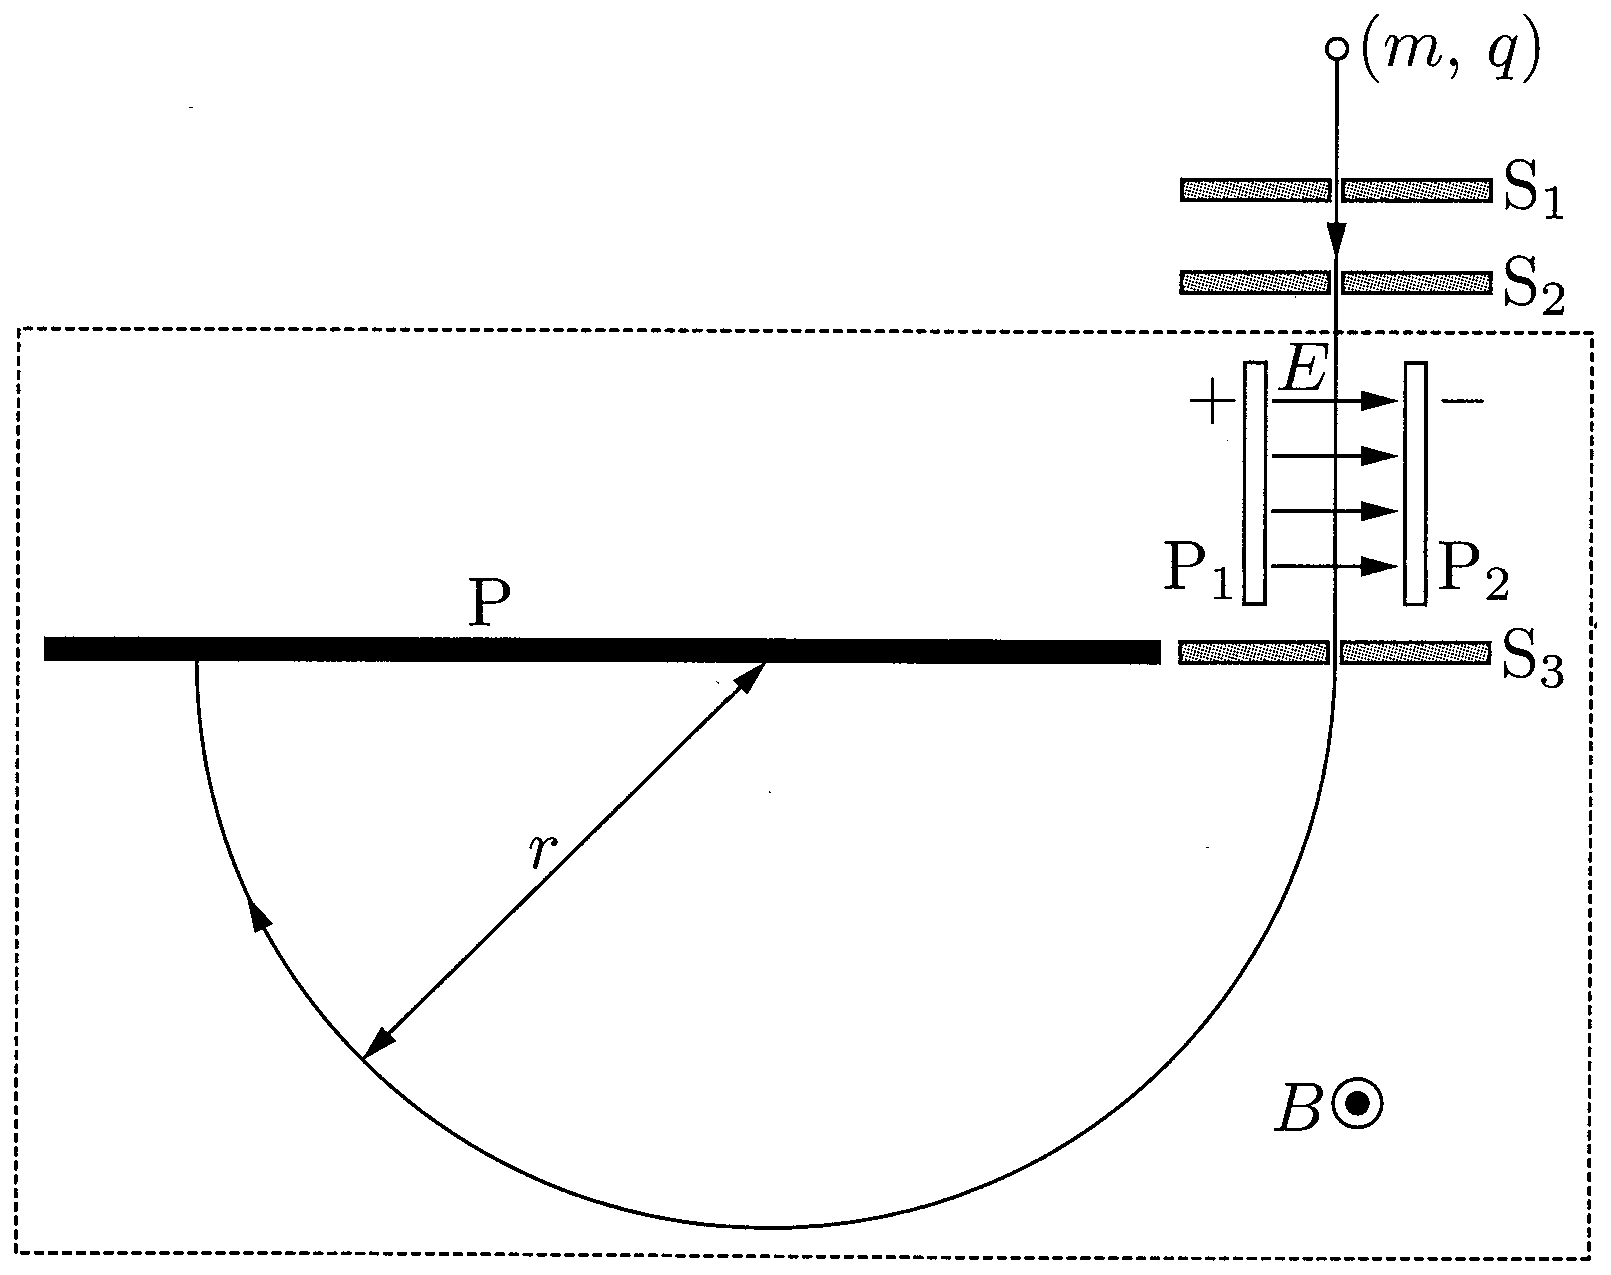
\includegraphics[keepaspectratio,width=60mm]{fig/n29_p95_zu.png}
\end{zuright}
\hspace{1zw}今，さまざまな質量$m\U{kg}$と電荷$q\U{C}$（$q>0$）をもった正の荷電粒子がスリット$\mathrm{S}_1$から入射し，スリット$\mathrm{S}_2$を通過して平行平板電極の間の電場の中に垂直に入射した．この荷電粒子の速さを$v\U{m/s}$とすると，荷電粒子には電場から大きさ\framebox[4zw]{\rule{0pt}{1.1zw}1}のクーロン力が\framebox[4zw]{\rule{0pt}{1.1zw}2}の向きに働き，一方，磁場により大きさ\framebox[4zw]{\rule{0pt}{1.1zw}3}のローレンツ力が\framebox[4zw]{\rule{0pt}{1.1zw}4}の向きに働く．したがって速さが$v_0=$\framebox[4zw]{\rule{0pt}{1.1zw}5}の荷電粒子はまっすぐ進んでスリット$\mathrm{S}_3$を通過するが，それ以外の速さを持った荷電粒子はスリット$\mathrm{S}_3$を通過することができない．
\par
\hspace{1zw}また，スリットを通過した荷電粒子は，半径$r=$\framebox[4zw]{\rule{0pt}{1.1zw}6}の円軌道を描いて乾板$\mathrm{P}$に到達する．したがって$r$を測定すれば比電荷が求まることになる．

\filbreak
\Rank{C問題}

\Mon{ホール効果}

\begin{zuright}{52mm}
\hspace{1zw}次の\framebox[4zw]{\rule{0pt}{1.1zw}1}から\framebox[4zw]{\rule{0pt}{1.1zw}7}に当てはまる適当な語句および数値を入れよ．
\par
\hspace{1zw}右図のように，断面が$a\U{m}\times b\U{m}$の長方形である半導体柱に，$z$軸正方向へ強さ$I\U{A}$の電流を流した．半導体には，負電荷である電子が半導体中を移動することで電流となるものと，正電荷である正孔（ホール）が半導体中を移動することで電流となるものの2タイプがあるが，ここでは後者のタイプの半導体を考え，
\zusep
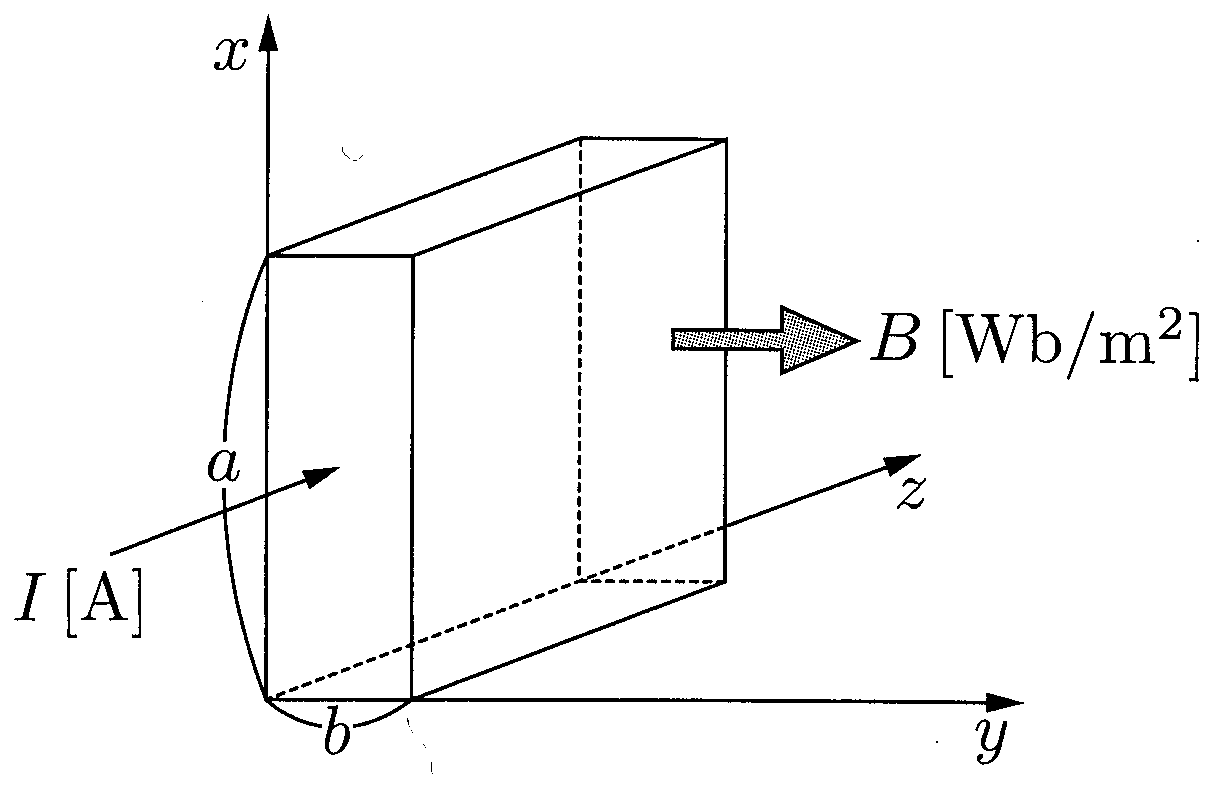
\includegraphics[keepaspectratio,width=50mm]{fig/n29_p96_zu.png}
\end{zuright}
さらにこの半導体柱には正の電荷$+q\U{C}$の荷電粒子（正孔）が，単位体積あたり$n\U{個/m^3}$だけ存在し，これらの粒子すべてが$z$軸正方向へ同一の速さ$\overline{v}\U{m/s}$で運動することで電流が流れているとする．このとき，流れている電流の強さが$I\U{A}$であることから，$\overline{v}=$\framebox[4zw]{\rule{0pt}{1.1zw}1}と表せる．今，ここで$y$軸正方向に磁束密度$B\U{Wb/m^2}$の一様な磁場をかけると，荷電粒子は磁場から\framebox[4zw]{\rule{0pt}{1.1zw}2}方向に$f=$\framebox[4zw]{\rule{0pt}{1.1zw}3}の力を受け，この半導体の上面には\framebox{\rule{0pt}{1.1zw}\,4：正，負\,}電荷が，また下面にはそれと逆の電荷が蓄積される．その結果，これらの蓄積した電荷により半導体内には\framebox[4zw]{\rule{0pt}{1.1zw}5}方向に電場が発生する．これをホール効果という．ある程度の電荷が蓄積されると，正孔がこの電場から受ける力と，磁場による力$f$とが打ち消し合うようになり，その結果，正孔は$z$軸正方向のみに移動していき，この方向にだけ一様な電流が流れることになる．このときの電場の強さ$E\U{V/m}$は$E=$\framebox[4zw]{\rule{0pt}{1.1zw}6}と表すことができる．またこのときの上下面間の電位差は$V=$\framebox[4zw]{\rule{0pt}{1.1zw}7}となり，これをホール電圧という．

\Mon{電場中の荷電粒子の運動}

\begin{zuright}{62mm}
\hspace{1zw}右図のように距離$d\U{m}$だけ離して平行に二つの金属板$\mathrm{P}$，$\mathrm{Q}$を置き，$\mathrm{P}$と$\mathrm{Q}$との電位差を$V\U{V}$に保つ．$\mathrm{A}$，$\mathrm{B}$は$\mathrm{P}$にあけられた小さな穴で，この間の距離は$l\U{m}$である．穴$\mathrm{A}$から$\mathrm{A}$，$\mathrm{B}$を含み$\mathrm{P}$に垂直な平面内で，右図のように$\mathrm{P}$の面と角$\theta\U{rad}$をなす向きに，速さ$v\U{m/s}$で電子を入射させる．電子の質量を$m\U{kg}$，電荷を$-e\U{C}$として以下の設問に答えよ．ただし電子に働く重力による効果は無視できるものとする．
\zusep
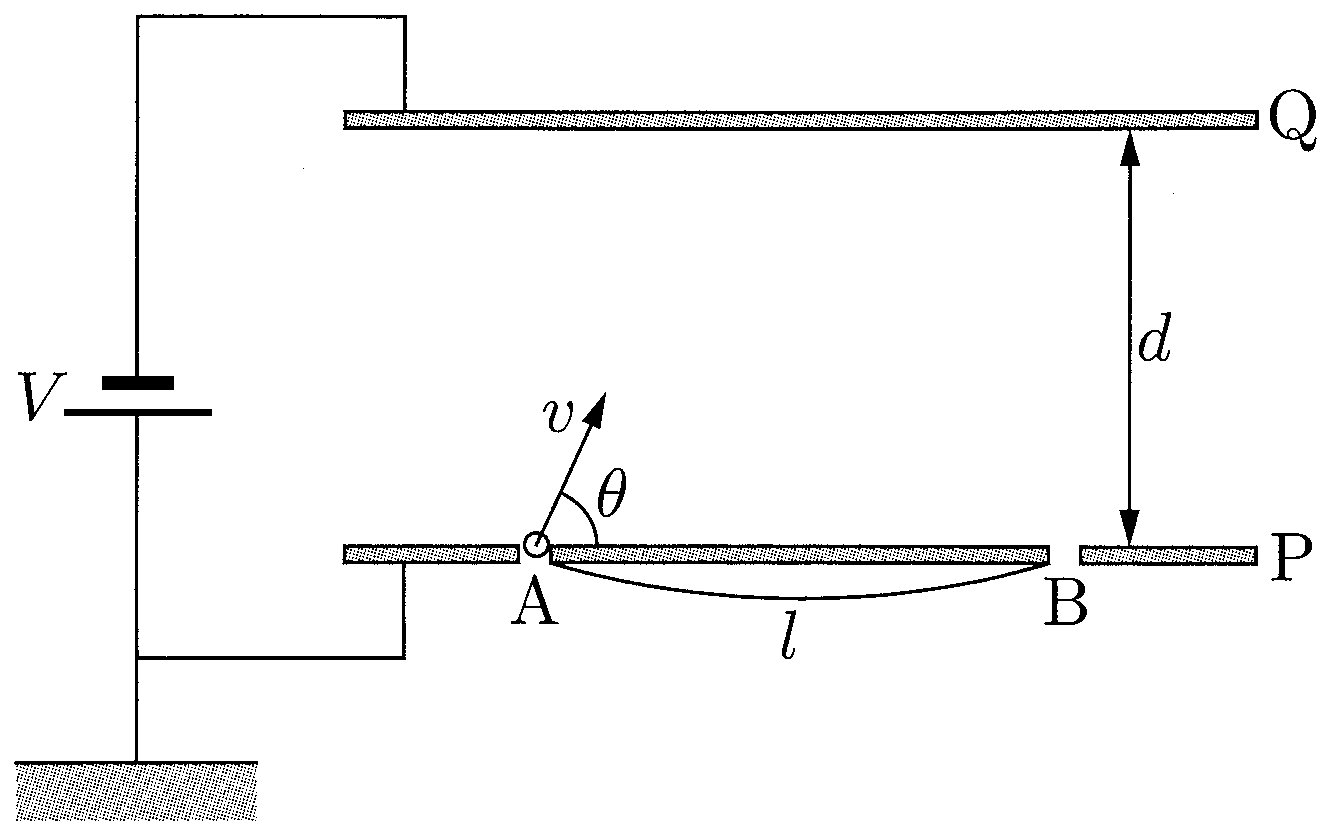
\includegraphics[keepaspectratio,width=60mm]{fig/n29_p97_zu.png}
\end{zuright}
\begin{komon}
\ko{1} $\mathrm{PQ}$間に生じる電場の向きと大きさを求めよ．
\ko{2} 電子が$\mathrm{Q}$に衝突しないための条件を求めよ．
\ko{3} 電子が$\mathrm{Q}$に衝突せずに，穴$\mathrm{B}$から外へ出るための$v$の値および$\tan\theta$の値の範囲を求めよ．
\end{komon}

\Mon{サイクロトロン}

\begin{zuright}{52mm}
\hspace{1zw}次の\framebox[4zw]{\rule{0pt}{1.1zw}1}〜\framebox[4zw]{\rule{0pt}{1.1zw}5}の空欄に適する式および語句を埋めよ．なお，\framebox[4zw]{\rule{0pt}{1.1zw}3}については，語群の中から選べ．
\par
\hspace{1zw}磁場中を磁場の向きと垂直な面内で運動している荷電粒子は円軌道を描く．磁束密度を$B\U{Wb/m^2}$，粒子の質量，電荷をそれぞれ$m\U{kg}$，$q\U{C}$（ただし$q>0$とする），粒子の速さを$v\U{m/s}$とすれば，粒子の円運動の半径は$r=$\framebox[4zw]{\rule{0pt}{1.1zw}1}と表せ，円運動の周期$T\U{s}$は$T=$\framebox[4zw]{\rule{0pt}{1.1zw}2}と$r$，$v$によらない形で表すことができる．
\zusep
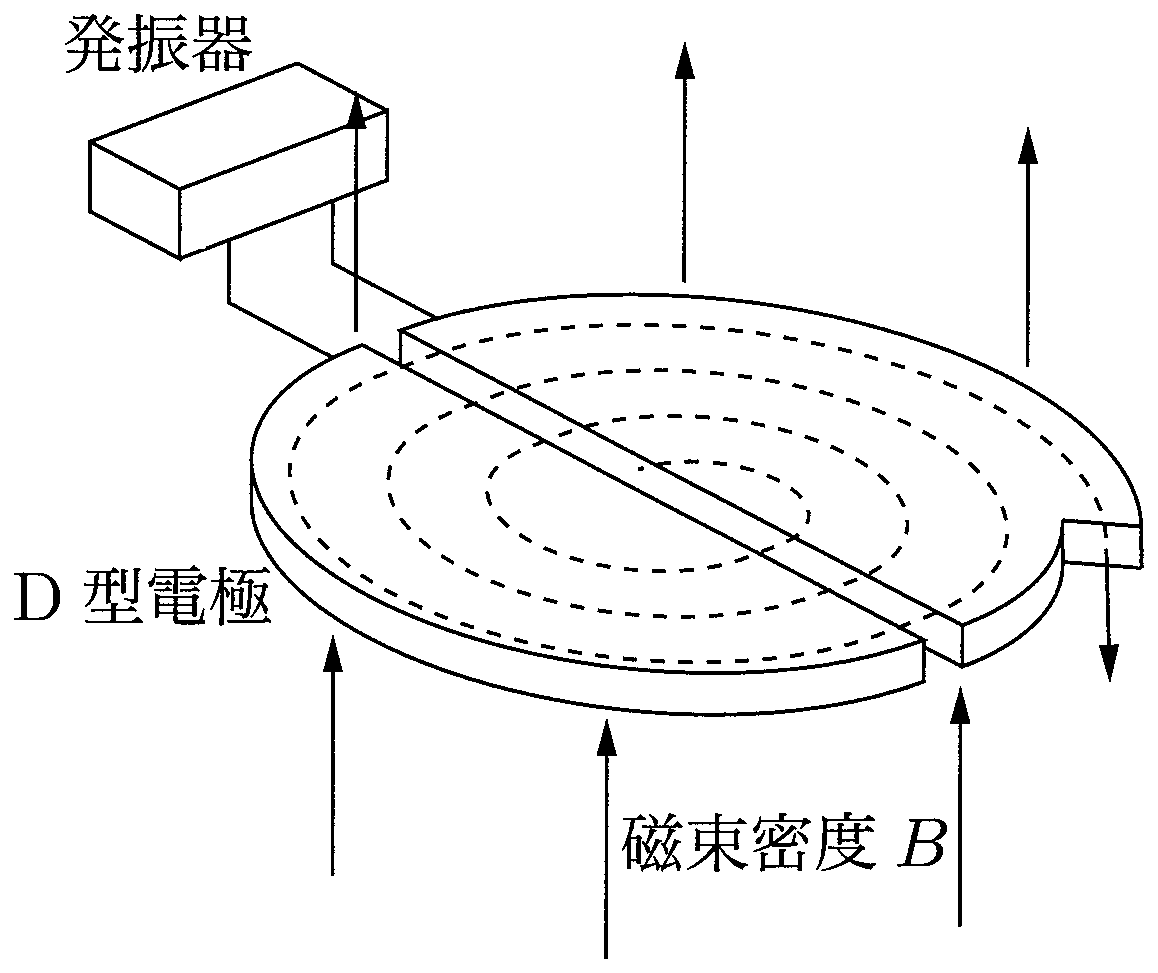
\includegraphics[keepaspectratio,width=50mm]{fig/n29_p98_zu.png}
\end{zuright}
\hspace{1zw}今，磁極間の真空中に，右図のような二つの向かい合ったD形の中空電極を入れ，これに発振器を用いて高周波数の交流電圧をかけて，電極の正，負を交互に変化させる．交流電圧の周期を粒子の回転の周期と\framebox{\rule{0pt}{1.1zw}\,3：等しく，半分に，2倍に\,}すると，一度電極のすき間で加速された粒子は半回転して再び加速されることになり，これを何回も繰り返すことができる．これが粒子加速器，サイクロトロンの原理である．サイクロトロンを用いて，原子核の性質を調べることができる．
\par
\hspace{1zw}さて周波数$f_0\U{Hz}$，D形電極内の粒子の最大軌道半径が$R\U{m}$のサイクロトロンがある．このサイクロトロンで質量$M\U{kg}$，電荷$Q\U{C}$（$>0$）の粒子を加速するために必要な磁束密度は$B_0=$\framebox[4zw]{\rule{0pt}{1.1zw}4}であり，このとき出てくる粒子のエネルギーは$E=$\framebox[4zw]{\rule{0pt}{1.1zw}5}である．

\newpage

%%%%%%%%%%%%%%%%%%%%  解答  %%%%%%%%%%%%%%%%%%%%
\KaiTitle{第29回　電場・磁場中の荷電粒子の運動}
\setlength{\columnseprule}{0.4pt}
\begin{multicols}{2}
\raggedcolumns

\Rank{A問題}
\MonN{90}{基本公式の確認}\par\nopagebreak
\begin{sisin}
電磁力$f=IBl\sin\theta\U{N}$およびローレンツ力$f=qvB\sin\theta\U{N}$を適宜利用して考えよう．磁場の向きと電流の向きもしくは荷電粒子の速度の向きが直交していない場合には，直交成分を取り出して計算すること．なお，これらの式はいずれも磁束密度$B$を利用して記述されている．磁場の強さ$H$として与えられている場合には磁束密度に換算してから代入すること．
\end{sisin}
\KaiHead
\begin{komon}
\ko{1} \[\begin{aligned}
         f&=IBl=I\cdot(\mu_0H)\cdot l\\
          &=2.0\cdot 4\pi\times 10^{-7}\cdot 20\cdot 0.10\\
          &\fallingdotseq 5.0\times 10^{-6}\U{N}\Ans
       \end{aligned}\]
\ko{2} 電子の半径方向の運動方程式は$m\dfrac{v^2}{r}=evB$であるから，電子の軌道半径は
       \[\begin{aligned}
         r&=\frac{mv}{eB}=\frac{9.1\times 10^{-31}\cdot 1.6\times 10^7}{1.6\times 10^{-19}\cdot 1.4}\\
          &=6.5\times 10^{-5}\U{m}\Ans
       \end{aligned}\]
       また，周期は
       \[\begin{aligned}
         T&=\frac{2\pi r}{v}=\frac{2\times 3.14\times 6.5\times 10^{-5}}{1.6\times 10^7}\\
          &\fallingdotseq 2.6\times 10^{-11}\U{s}\Ans
       \end{aligned}\]
\end{komon}

\Rank{B問題}
\MonN{91}{複数の点電荷による電位の合成}\par\nopagebreak
\begin{sisin}
電場の場合は向きを考えてベクトル合成する必要があるのに対して，電位の場合は向きを考える必要はなく，単純に数値の和を取ればよい（スカラー合成）．
% 原本は「前回の［4］の問題と見かけ上は似ているが」（旧回の番号なので外した）．
(2)は，無限遠方にたどり着けるかどうかをエネルギー保存則で判定する（29.1）．
\end{sisin}
\KaiHead
\begin{komon}
\ko{1} 各点の電位は，$\mathrm{A}$が作る電位と$\mathrm{B}$が作る電位とを単純和すれば求められる．よって，
       \[\begin{aligned}
         V_{\mathrm{P}}&=k\frac{+q}{d-l}+k\frac{-q}{d+l}=\frac{2kql}{d^2-l^2}\U{V}\\
         V_{\mathrm{Q}}&=k\frac{+q}{d+l}+k\frac{-q}{d-l}=-\frac{2kql}{d^2-l^2}\U{V}\\
         V_{\mathrm{R}}&=k\frac{+q}{\sqrt{d^2+l^2}}+k\frac{-q}{\sqrt{d^2+l^2}}=0\U{V}
       \end{aligned}\]
       \hspace*{\fill}$\cdots$(答)
\ko{2} 無限遠方に飛び去った際に，無限遠方にて物体が持つ速さを$v\U{m/s}$とおく．物体には保存力である静電気力のみが作用するため，力学的エネルギー保存則を適用することができる．無限遠方の電位は$0\U{V}$になることに注意して，$\mathrm{Q}$点と無限遠方との間に力学的エネルギー保存則を適用すると，
       \[\frac{1}{2}mv_0^2+(+q)\cdot V_{\mathrm{Q}}=\frac{1}{2}mv^2+(+q)\cdot 0\]
       である．実際に無限遠方に到達するためには，この式の$v$が存在することが必要であり，そのためには
       \[\frac{1}{2}mv_0^2+(+q)\cdot V_{\mathrm{Q}}\geqq 0\]
       でなければならない．よってこれを整理すると，
       \[v_0\geqq 2q\sqrt{\frac{kl}{m(d^2-l^2)}}\U{m/s}\Ans\]
       以上あれば無限遠方に飛び去ることができる．
       \begin{chuu}
       厳密には，$\mathrm{Q}$から無限遠までの途中で電位が$V_{\mathrm{Q}}$より高くならないことも必要である．$x>d$では$-q$に近い負の電位が$0$に向かって単調に上がっていくので，途中で追い返されることはなく，上の条件で十分である．
       \end{chuu}
\end{komon}

\MonN[\Sitei]{92}{磁場中の荷電粒子の運動}\par\nopagebreak
\begin{sisin}
磁場に入射した荷電粒子の運動がどうなるかについてしっかり覚えておくこと．二つのパターンに分かれており，\MARU{1}磁場に対して垂直な方向に入射した場合には等速円運動を，\MARU{2}磁場に対して斜めの方向に入射した場合にはらせん運動を行う．いずれの場合でも磁場に平行な方向と，磁場に対して垂直な面内方向とに速度・力を成分分解して考え，磁場に対して垂直な面内に対して等速円運動の運動方程式を立てて考える．
\end{sisin}
\KaiHead
\begin{komon}
\ko{1} 運動中，粒子に働くローレンツ力は速度に対して常に垂直であるから，粒子に対して仕事をなさず，粒子の速さは一定値$v\U{m/s}$である．よってローレンツ力は常に一定の大きさ$qvB\U{N}$で，かつ粒子の速度に対して垂直であるから，粒子はこの面内で等速円運動を行う．この正電荷を持つ荷電粒子が受けるローレンツ力の向きを考えると，次図のような向きの円軌道を描くことが分かる．
       \begin{center}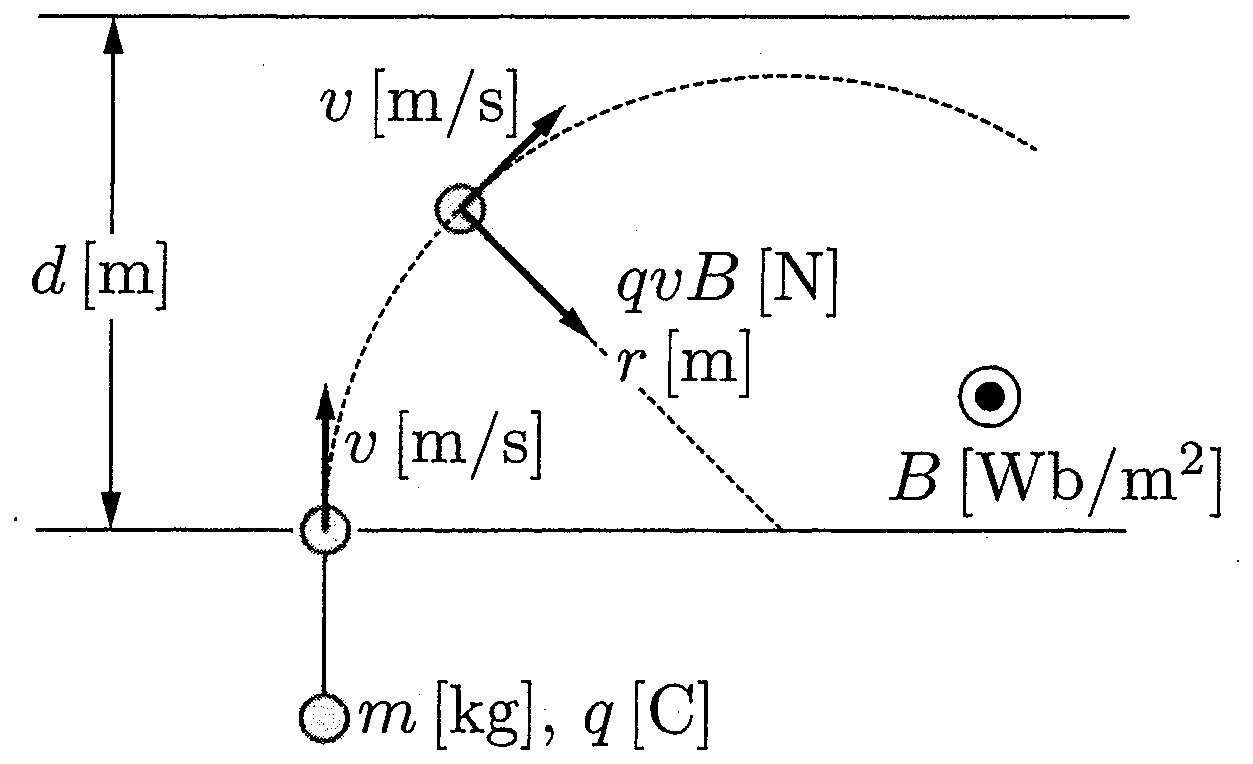
\includegraphics[keepaspectratio,width=56mm]{fig/n29_a92_zu1.png}\end{center}
       よって，この軌道半径を$r\U{m}$とすれば，粒子の半径方向の運動方程式は$m\dfrac{v^2}{r}=qvB$であり，これを解いて，$r=\dfrac{mv}{qB}\U{m}$である．前図から分かるように，$d>r$であればこの粒子が対極に到達しない．よって，求める条件は，
       \[d>\frac{mv}{qB}\U{m}\Ans\]
\ko{2} $d$を$d\leqq r$の範囲で変化させるとき，円軌道の半径$r=\dfrac{mv}{qB}$は$d$を変化させても変わらないので，最も磁場中での運動時間が長くなるのは次図より明らかに$d=r$のときである．
       \begin{center}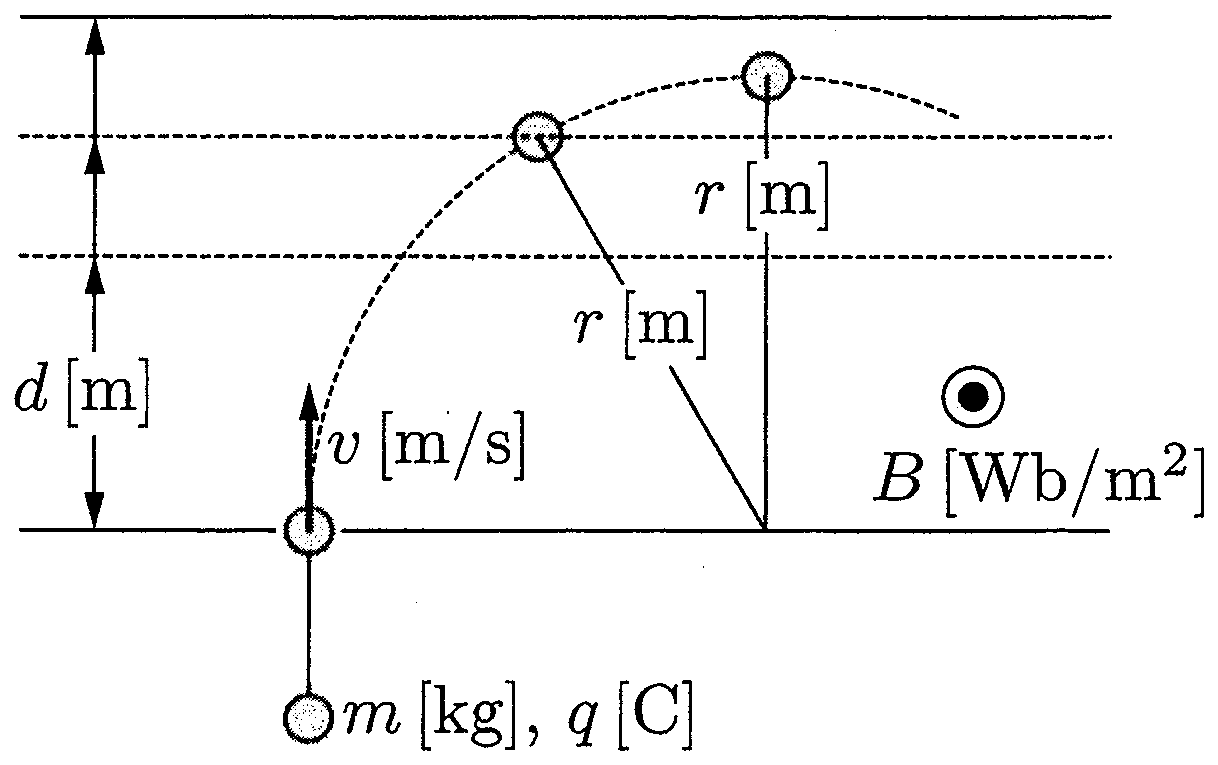
\includegraphics[keepaspectratio,width=56mm]{fig/n29_a92_zu2.png}\end{center}
       よって，
       \[d=\frac{mv}{qB}\U{m}\Ans\]
       のとき，対極への到達時間が最も長くなる．またこのとき，対極へは円弧の$\dfrac{1}{4}$を描いて到達するので，その所要時間は，
       \[t_{\max}=\frac{2\pi r}{v}\times\frac{1}{4}=\frac{\pi m}{2qB}\U{s}\Ans\]
\end{komon}

\MonN{93}{磁場中での電子のらせん運動}\par\nopagebreak
\begin{sisin}
コイル内には$+z$の向きに一様な磁場が発生するので，これに斜めに入射した荷電粒子は磁場中でらせん軌道を描く．らせん運動の取り扱いは，磁場に平行な方向と，磁場に垂直な面内とに分けるのが基本（例題28）．磁場に垂直な面内に対して運動方程式を立てて処理しよう．
\end{sisin}
\KaiHead
\begin{komon}
\ko{1} 電池をつないだことにより，コイルには$\mathrm{P}$から$\mathrm{Q}$へ上がっていく向きに電流が流れる．よって，コイルの巻きの向きを考えると，右ねじの法則よりコイル内には{\gtfamily $+z$の向き}に一様な磁場が発生する．\Ans
       コイルの単位長さあたりの巻き数$n_0$が$\dfrac{N}{l}$であることに注意して，
       \[H=n_0I=\frac{N}{l}I\U{A/m}\Ans\]
\ko{2} (1)で求めた磁場を磁束密度に換算すると，$B=\mu_0H=\mu_0\dfrac{N}{l}I\U{Wb/m^2}$である．

       磁場に入射した荷電粒子の運動を，$xy$面内方向と$z$軸方向とに分けて考えると，磁場に平行なので$z$軸方向の速度成分にはローレンツ力はかからず，また$xy$面内方向の速度成分にかかるローレンツ力はフレミングの左手の法則より$xy$面内の方向になるので，$z$軸方向には力が作用せず，$z$軸方向の速度は$v_{/\!/}$の一定値に保たれる．

       また，$xy$面内方向の運動について考えると，初速度の向きとローレンツ力の向き（この粒子は電子ゆえ負電荷である）を考えて，図のような円軌道を描くと分かる．
       \begin{center}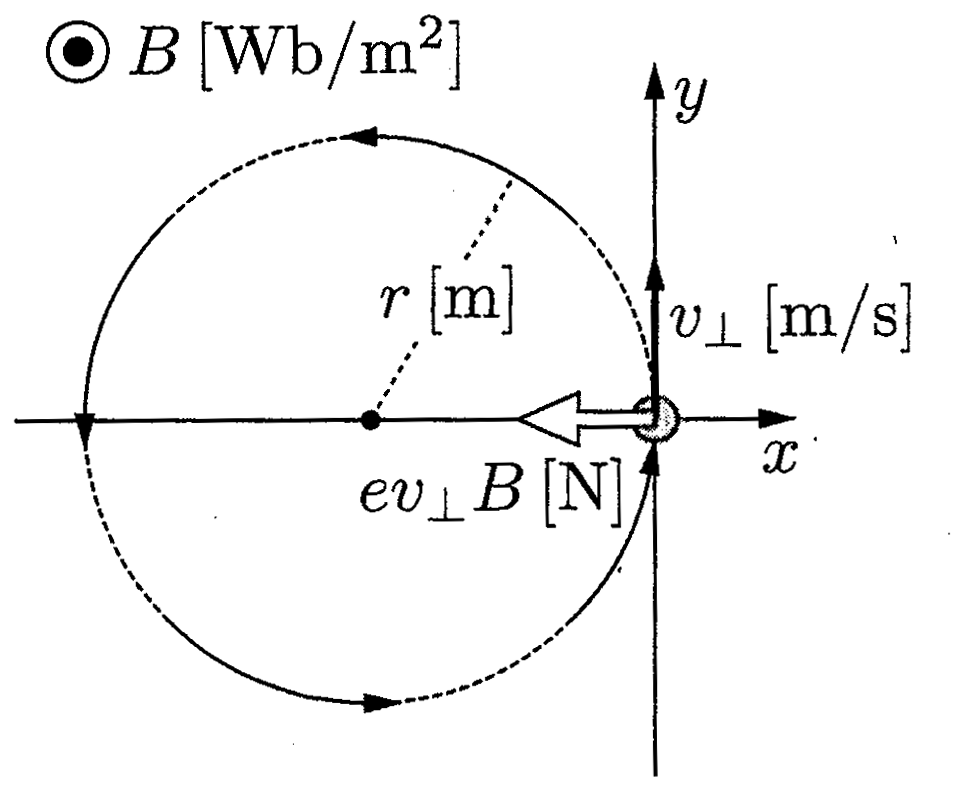
\includegraphics[keepaspectratio,width=50mm]{fig/n29_a93_zu.png}\end{center}
       電子の$xy$面内，円運動中心向きの運動方程式は$m\dfrac{v_\perp^2}{r}=ev_\perp B$であるからこれを解いて，
       \[r=\frac{mv_\perp}{eB}=\frac{mv_\perp l}{e\mu_0NI}\U{m}\]
       また，前図よりらせん運動を$xy$平面に投影したときの円軌道の中心点は$(-r,0,0)$であるから上の結果を代入して，
       \[\Bigl(-\frac{mv_\perp l}{e\mu_0NI},\ 0,\ 0\Bigr)\U{m}\Ans\]
       この粒子が$\mathrm{O}$点を出発してから$\mathrm{S}$点に到達するまでに荷電粒子は円軌道を一周しているので，求めるべき所要時間は，
       \[T=\frac{2\pi r}{v_\perp}=\frac{2\pi ml}{e\mu_0NI}\U{s}\Ans\]
\ko{3} $\mathrm{O}$点を出発してから$\mathrm{S}$点に到達するまでの$T$の間，$z$軸方向には$v_{/\!/}$の一定速度で運動する．よって，らせんのピッチは
       \[\overline{\mathrm{OS}}=v_{/\!/}T=\frac{2\pi mlv_{/\!/}}{e\mu_0NI}\U{m}\Ans\]
\end{komon}

\MonN[\Sitei]{94}{トムソンの実験}\par\nopagebreak
\begin{sisin}
上側極板に正電荷が溜まっているので，極板間を負電荷の電子が通過するときは進行方向が上側にねじ曲げられてそれる．当然，上側極板の正電荷が大きければ大きいほど，電子線のねじ曲がり方は大きくなる．このことをよく考えれば，問題文にある，「輝点が一瞬消え，短時間後にある定点$\mathrm{P}$が光るようになる」が何を意味するのかが分かるはず．
\end{sisin}
\KaiHead
\begin{komon}
\ko{1} $\mathrm{K}$，$\mathrm{H}$間のエネルギー保存則より，
       \[\frac{1}{2}m\cdot 0^2+(-e)\cdot(-V_0)=\frac{1}{2}mv_0^2+(-e)\cdot 0\]
       これを解いて，
       \[\begin{aligned}v_0&=\sqrt{\frac{2eV_0}{m}}=1.02\times 10^7\\&\fallingdotseq 1.0\times 10^7\U{m/s}\Ans\end{aligned}\]
\ko{2} 極板$\mathrm{D}$に正電荷を与えると，極板間に下向きの電場が生じるため，電子が極板間を通過するときに上向きの力を受け，電子線は上へそれる．
       \begin{center}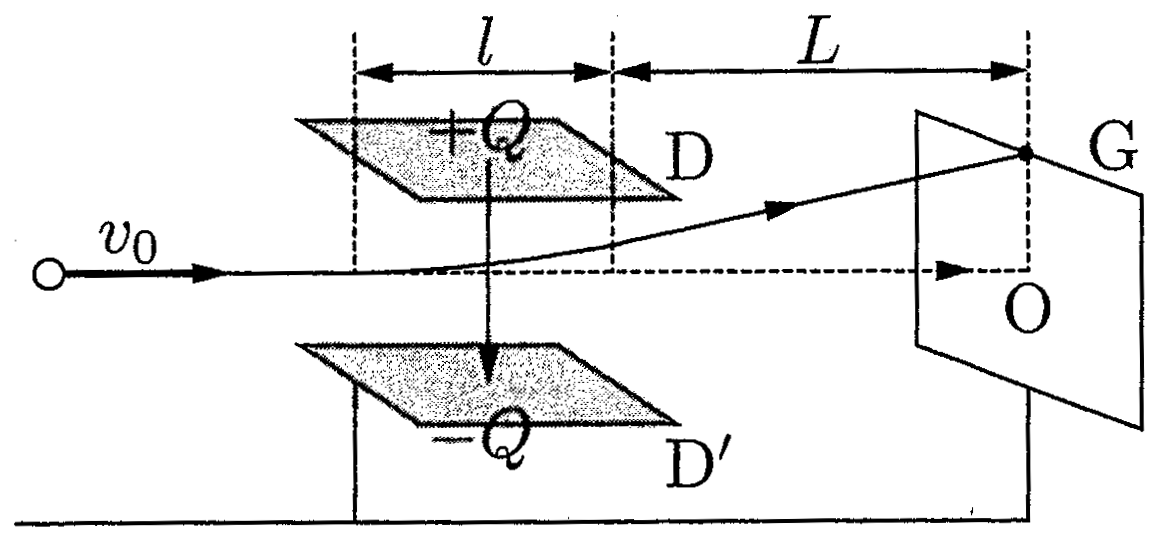
\includegraphics[keepaspectratio,width=56mm]{fig/n29_a94_zu1.png}\end{center}
       偏向の度合は極板$\mathrm{D}$に与えた正電荷が大きければ大きいほど大きくなるが，正電荷がある大きさを超えてしまうと（$Q>Q_0$）電子線は極板のすき間を通過せずに極板$\mathrm{D}$に衝突してしまう．
       \begin{center}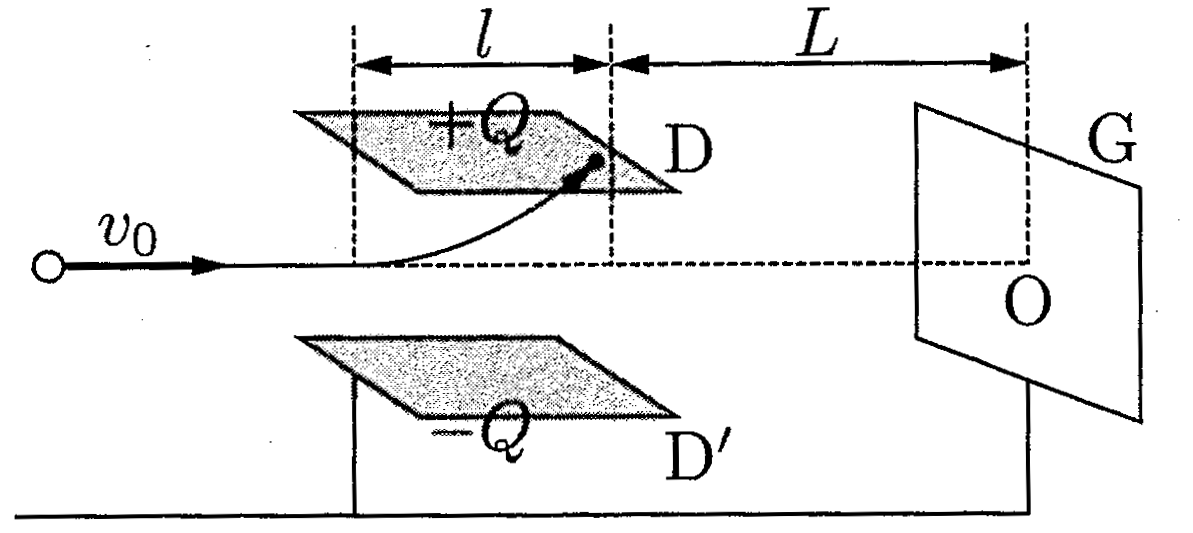
\includegraphics[keepaspectratio,width=56mm]{fig/n29_a94_zu2.png}\end{center}
       この場合，極板$\mathrm{D}$に衝突した電子は極板$\mathrm{D}$上の電荷を打ち消していくので，時間がたつにつれて極板$\mathrm{D}$上の電荷は小さくなっていき，電子線の偏向の度合は弱まる．そして電子線が極板$\mathrm{D}$の端をかすめるようになると電子は極板$\mathrm{D}$にぶつからず，スクリーン上に輝点を生じるようになる．\Ans
       \begin{center}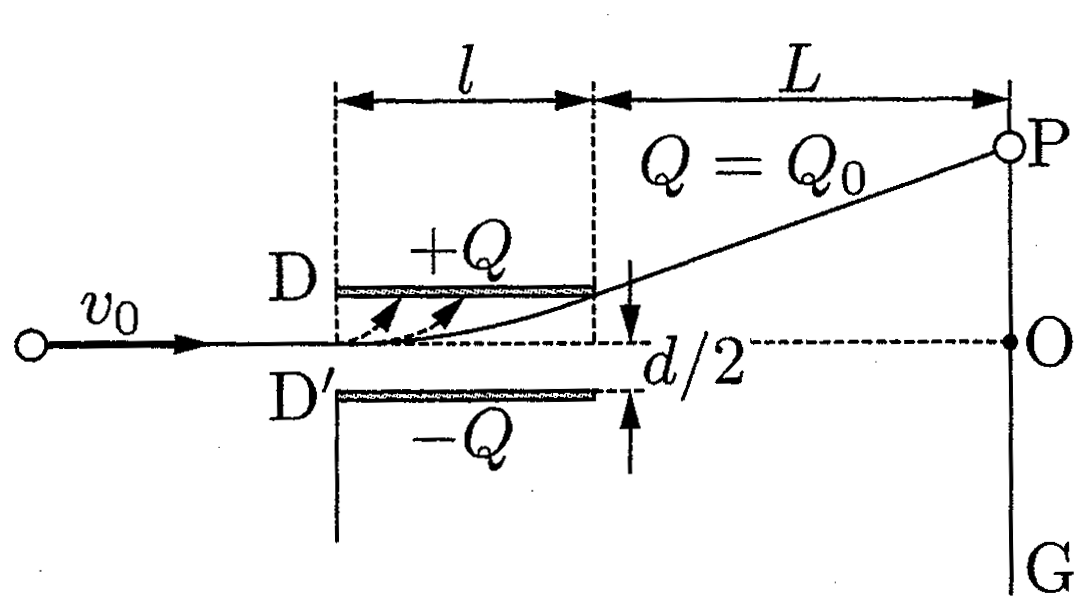
\includegraphics[keepaspectratio,width=56mm]{fig/n29_a94_zu3.png}\end{center}
\ko{3} (2)から分かるように，定点$\mathrm{P}$の位置は$Q$の値にはよらない．また$Q_0$とは，この電荷を与えたときに電子線がぎりぎり極板$\mathrm{D}$の端をかすめるように進む場合の電荷に対応している．$Q=Q_0$の場合について考えると，平行平板コンデンサー$\mathrm{DD}^\prime$の電気容量は$C=\varepsilon_0\dfrac{l^2}{d}$であり，極板$\mathrm{DD}^\prime$間に作られる電場の強さは
       \[E=\frac{Q_0/C}{d}=\frac{Q_0}{\varepsilon_0l^2}\U{V/m}\]
       である．極板間で電子が鉛直上向きに持つ加速度の大きさを$a_y$とすると，極板間における電子の運動方程式は$ma_y=eE$ゆえ，$a_y=\dfrac{eQ_0}{m\varepsilon_0l^2}$．

       極板間を電子が通過するのに要する時間は，電子の水平方向の速度が変わらないことに着目して，$t_0=\dfrac{l}{v_0}$であり，電子線がぎりぎり極板$\mathrm{D}$の端をかすめるためには極板を通過しきる瞬間に上方向に$\dfrac{d}{2}$だけ動いていればよく，$\dfrac{1}{2}a_yt_0^2=\dfrac{d}{2}$が満たされていればよい．この条件式を解いて，
       \[\begin{aligned}
         Q_0&=\frac{m\varepsilon_0dv_0^2}{e}=\frac{m\varepsilon_0d}{e}\cdot\frac{2eV_0}{m}=2\varepsilon_0dV_0\\
         &=5.34\times 10^{-11}\fallingdotseq 5.3\times 10^{-11}\U{C}\Ans
       \end{aligned}\]
       また，このとき極板間を通過しきる瞬間の，水平方向および鉛直方向の速さはそれぞれ$v_x=v_0$，$v_y=a_yt_0$であるから，偏向角を$\theta$とすると，
       \[\tan\theta=\frac{v_y}{v_x}=\frac{a_yt_0}{v_0}=\frac{a_yt_0^2}{l}=\frac{d}{l}\]
       である．次図の幾何学的関係を利用して，
       \begin{center}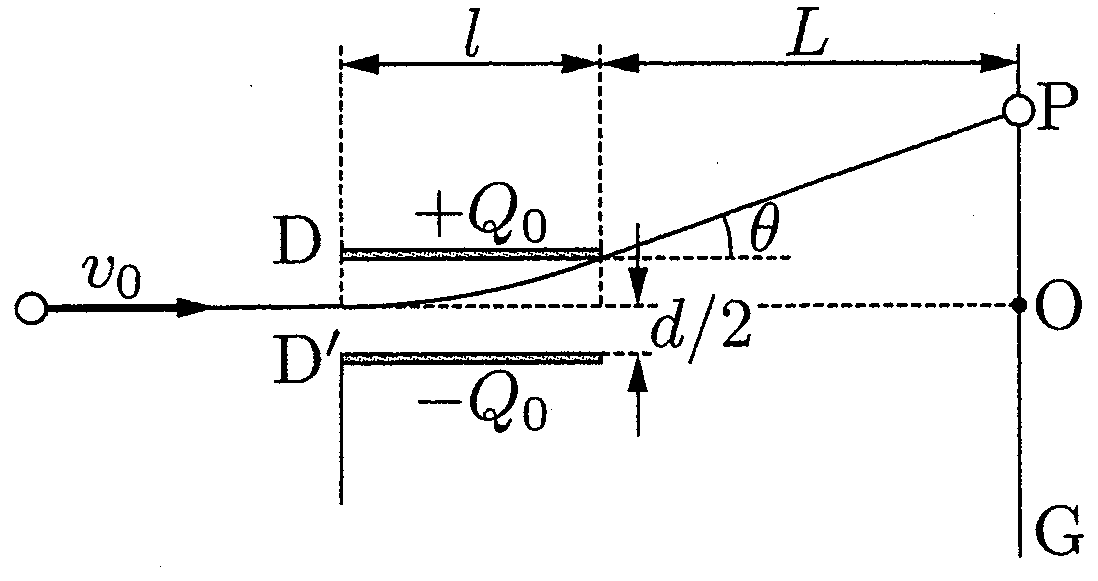
\includegraphics[keepaspectratio,width=56mm]{fig/n29_a94_zu4.png}\end{center}
       \[\begin{aligned}
         \overline{\mathrm{OP}}&=\frac{d}{2}+L\tan\theta=\Bigl(\frac{1}{2}+\frac{L}{l}\Bigr)d=0.105\\
         &\fallingdotseq 1.1\times 10^{-1}\U{m}\Ans
       \end{aligned}\]
       \begin{chuu}
       $Q_0$の値を計算する際に$v_0$に(1)の数値を直接代入しなかったのは計算を容易にするためであり，それ以上の理由はない（$Q_0=2\varepsilon_0dV_0$という式は特別に意味のある式ではない）．
       \end{chuu}
\ko{4} $Q=1.0\times 10^{-10}\U{C}$の電荷を与えた場合には(2)で述べたように，初め，電子線が極板$\mathrm{D}$へ衝突して吸収されていき，極板$\mathrm{D}$の電荷が$Q_0=5.3\times 10^{-11}\U{C}$まで中和されると点$\mathrm{P}$に輝点を生じる．電子は毎秒$10^9$個ずつ送りこまれるので，極板$\mathrm{D}$の電荷が$Q_0$まで中和されるのに要する時間は，
       \[\begin{aligned}
         \frac{Q-Q_0}{1.6\times 10^{-19}}\times\frac{1}{10^9}&=0.293\\
         &\fallingdotseq 2.9\times 10^{-1}\U{s}\Ans
       \end{aligned}\]
\end{komon}

\MonN{95}{電場・磁場偏向}\par\nopagebreak
\begin{sisin}
本問は質量分析器と呼ばれる装置の原理図で，現在では物質の質量を求めるために利用されている．まず，スリット$\mathrm{S}_1$，$\mathrm{S}_2$により加速した粒子の進行方向を一方向に揃える．続いて磁場・電場の二つを組み合わせた$\mathrm{P}_1$，$\mathrm{P}_2$間の部分（速度選別器，29.5）である速度の粒子のみを選択的に取り出す．その後，磁場により円運動を行わせると質量の異なる粒子はスクリーン$\mathrm{P}$上の異なる点に到達する．かつてはこれを用いて同位体の分離・判別が行われた．
\end{sisin}
\KaiHead
\begin{komon}
\ko{1} $qE\U{N}$\Ans
\ko{2} $\mathrm{P}_1\to\mathrm{P}_2$（右）\Ans
\ko{3} $qvB\U{N}$\Ans
\ko{4} $\mathrm{P}_2\to\mathrm{P}_1$（左）\Ans
\ko{5} 電場による力と磁場からのローレンツ力がつり合うのは，$qE=qvB$より$v=\dfrac{E}{B}$のときであり，この速さを持つ荷電粒子のみが直進してスリット$\mathrm{S}_3$を通過することができる．よって，
       \[v_0=\frac{E}{B}\U{m/s}\Ans\]
       これより速い粒子は左へ，遅い粒子は右へねじ曲げられてそれる．
\ko{6} この荷電粒子はスリット$\mathrm{S}_3$を通過したのち，磁場からのローレンツ力によって等速円運動を行う．半径方向の運動方程式は$m\dfrac{v_0^2}{r}=qv_0B$であり，これを解いて，
       \[r=\frac{mv_0}{qB}=\frac{mE}{qB^2}\U{m}\Ans\]
\end{komon}

\Rank{C問題}
\MonN{96}{ホール効果}\par\nopagebreak
\begin{sisin}
向きに注意しながら考えていこう（29.5）．
\end{sisin}
\KaiHead
\begin{komon}
\ko{1} 電流の強さの定義より，$I=n\cdot q\cdot\overline{v}\cdot(ab)$が成立するので，
       \[\overline{v}=\frac{I}{nqab}\U{m/s}\Ans\]
\ko{2} 電流の担い手である正孔は正電荷を持っているので，電流が$+z$の向きに流れているということは正電荷である正孔が$+z$の向きに動いていることを意味する．よって，この荷電粒子に対して$+y$の向きに磁束密度をかけた場合，この荷電粒子はフレミングの左手の法則より
       \[-x\ \text{の向き}\Ans\]
       にローレンツ力を受ける．
\ko{3} \[f=q\cdot\overline{v}\cdot B=\frac{BI}{nab}\U{N}\Ans\]
\ko{4} このローレンツ力により正孔は図のように運動方向をねじ曲げられる．その結果，半導体柱の下面は正孔の蓄積によりプラスに帯電し，上面は取り残された負電荷によりマイナスに帯電する．
       \begin{center}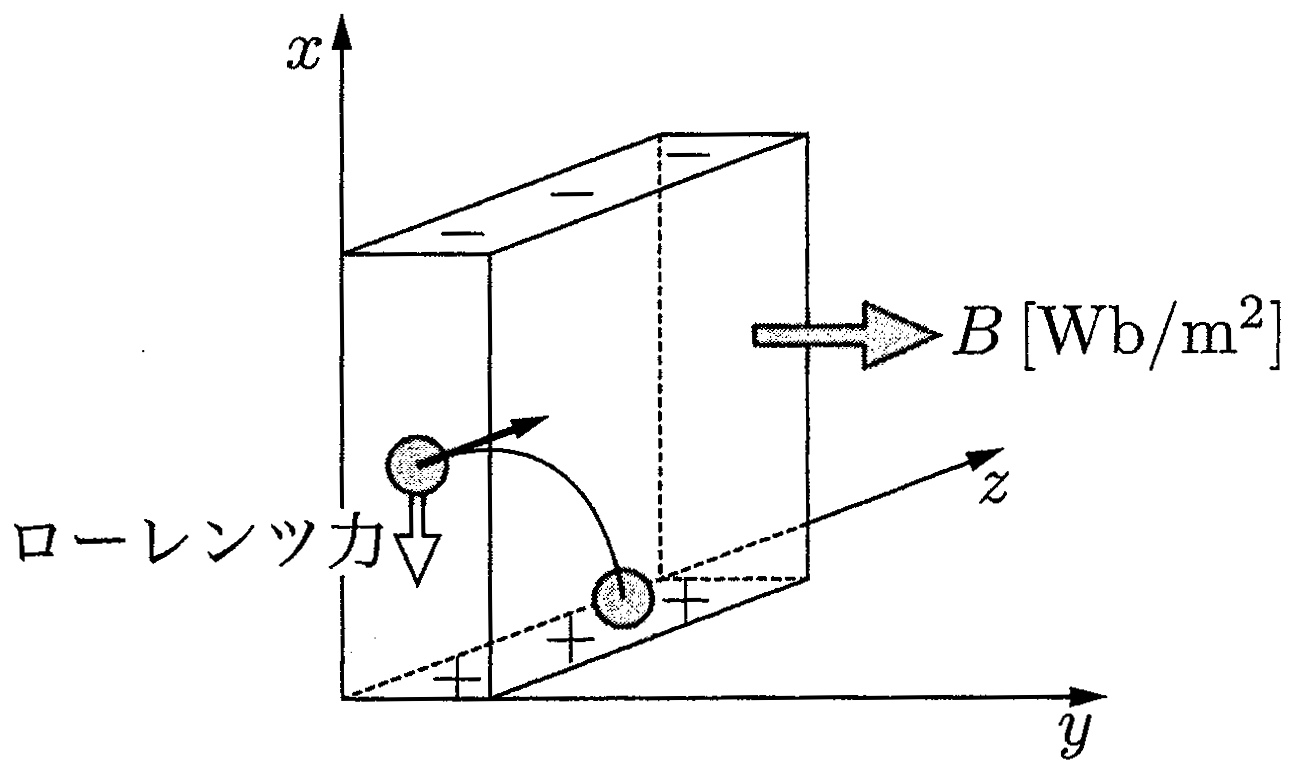
\includegraphics[keepaspectratio,width=56mm]{fig/n29_a96_zu.png}\end{center}
       よって，半導体上面に蓄積されるのは，{\gtfamily 負}電荷\Ans
\ko{5} (4)のようにして上面と下面に電荷が蓄積されると，正電荷→負電荷に向かう電場が発生する．前図を参照すれば，作られる電場の向きは
       \[+x\ \text{の向き}\Ans\]
\ko{6} 荷電粒子はこの電場からも力を受ける．ローレンツ力と電場からの力とがつり合うまで上面・下面の電荷が増加すると，もはや正孔は下面へ向かわなくなるため，それ以上の電荷の蓄積が起こらなくなる．このときの電場の強さを$E$とすると，力のつり合いの式$qE=q\overline{v}B$が成立する．これに(1)の結果を代入して解くと，
       \[E=\frac{BI}{nqab}\U{V/m}\Ans\]
\ko{7} 上面と下面の電位差は，
       \[V=E\cdot a=\frac{BI}{nqb}\U{V}\Ans\]
\end{komon}
\begin{bsHosoku}{参考}
問題文にもあるように，半導体中では電流の担い手が電子である場合と，正孔と呼ばれる正電荷である場合の2通りがある．しかし，単に電流を測定するだけではこの電子と正孔を区別することができない．しかし，ホール効果を利用すると，上面と下面の電位差は$V=\dfrac{BI}{nqb}$となり（負電荷の場合でも同じ結果になる），電流を担う荷電粒子の電気量$q$の正負がホール電圧$V$の正負として現れるので，これを測定することによって，電流の担い手が電子か正孔かを見分けることができる．
\end{bsHosoku}

\MonN{97}{電場中の荷電粒子の運動}\par\nopagebreak
\begin{sisin}
問題を見て，「この電子は$\mathrm{Q}$から反発を受けて$\mathrm{P}$に引っぱられるため放物線を描く」と直観的に理解して欲しい．電場中の荷電粒子の運動は，電場方向とそれに垂直な方向に分けて考えるのが基本（29.2）．軸を設定して考えよう．
% 原子編の章末問題［23］から移した（内容は完全に電磁気）．
\end{sisin}
\KaiHead
\begin{komon}
\ko{1} $\mathrm{PQ}$間の電位差が$V$，距離が$d$であるから，極板間にできる電場の大きさは，
       \[E=\frac{V}{d}\U{V/m}\Ans\]
       であり，向きは高電位側から低電位側，すなわち{\gtfamily $\mathrm{P}\to\mathrm{Q}$の向き}である．\Ans
\ko{2} $\mathrm{A}$点を原点として次図のように座標軸を取る．
       \begin{center}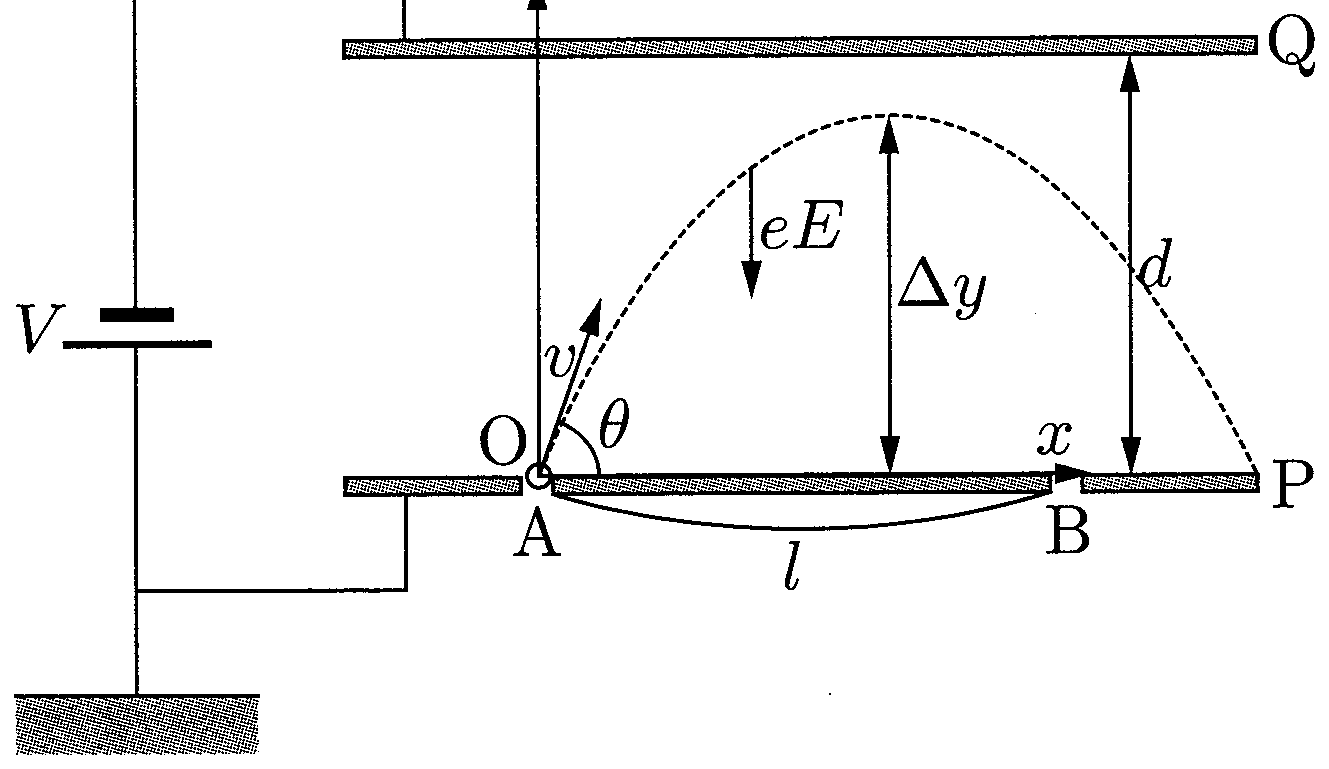
\includegraphics[keepaspectratio,width=56mm]{fig/n29_a97_zu.png}\end{center}
       このとき，極板間にある電子は電場と逆向き，すなわち$-y$方向に大きさ$eE$の力を受ける．よって，$y$軸方向の加速度を$a_y$として，運動方程式は$ma_y=-eE$より，$a_y=-\dfrac{eV}{md}$である．電子は$x$軸方向には力を受けないため，$x$軸方向には初速$v\cos\theta$を保つ等速度運動を行う．以上より，この電子は全体として放物運動を行う．

       $y$軸方向の運動のみに着目すると，最も$\mathrm{P}$から離れるとき$y$軸方向の速度が$0$となるので，そのときの$\mathrm{P}$からの距離を$\varDelta y$とすると（前図参照），等加速度直線運動であるから，$2a_y\cdot\varDelta y=0^2-(v\sin\theta)^2$が成立し，これを解いて，
       \[\varDelta y=\frac{md}{2eV}v^2\sin^2\theta\]
       である．電子が$\mathrm{Q}$に衝突しないためには，$\varDelta y<d$であればよい．これより，
       \[mv^2\sin^2\theta<2eV\Ans\]
\ko{3} $\mathrm{A}$点で入射してから最も$\mathrm{P}$から離れるまでに要する時間を$t_0$とすると，$t_0=\dfrac{v\sin\theta}{-a_y}=\dfrac{mdv\sin\theta}{eV}$である．また，最も$\mathrm{P}$から離れた点に達してから再び$\mathrm{P}$に戻ってくるまでに要する時間も，運動の対称性より$t_0$である．この間，電子は$x$軸方向には等速度運動を行っているので，再び$\mathrm{P}$に戻ってきたときの$x$座標は，
       \[x=v\cos\theta\cdot 2t_0=\frac{2mdv^2\sin\theta\cos\theta}{eV}\]
       である．電子がちょうど穴$\mathrm{B}$から外へ出るためには$x=l$であればよい．これを解いて，
       \[v=\sqrt{\frac{eVl}{2md\sin\theta\cos\theta}}\U{m/s}\Ans\]
       また，$\mathrm{Q}$に衝突しないためには(2)より$mv^2\sin^2\theta<2eV$が必要であった．上の$v$の場合についてこの条件式を解くと，
       \[\tan\theta<\frac{4d}{l}\Ans\]
\end{komon}

\MonN{98}{サイクロトロン}\par\nopagebreak
\begin{sisin}
原子物理で利用される粒子加速装置の一つ，サイクロトロンについて問う問題である（29.5）．磁場中に荷電粒子を入射させると等速円運動を行うが，本問のような二つのD型中空電極の内部でこの等速円運動を行わせる際，すき間（ギャップ）の部分に電場をかけるとギャップ部分で荷電粒子は加速され，粒子の運動エネルギーが増大する．例えば荷電粒子が正の電荷を持つ場合，荷電粒子が手前のDから奥のDへとギャップを通過する際に，手前のDを高電位に，奥のDを低電位にしておけば荷電粒子はギャップ通過の際に加速される．逆に，荷電粒子が奥のDから手前のDへとギャップを通過する際には，手前のDを低電位に，奥のDを高電位にしておけばよい．つまり，この荷電粒子がギャップを通過するごとに二つのDの電位を交互に正負反転させればギャップ通過のたびに荷電粒子を加速することができる（次図参照）．
\begin{center}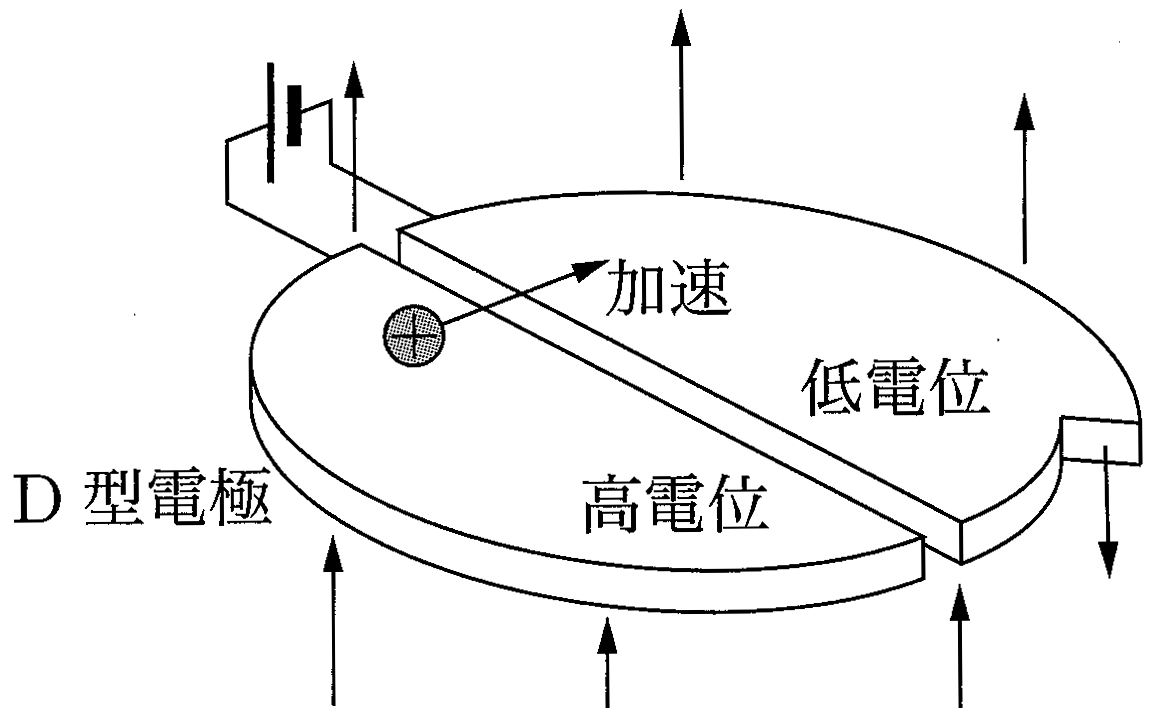
\includegraphics[keepaspectratio,width=52mm]{fig/n29_a98_zu1.png}\\[1mm]
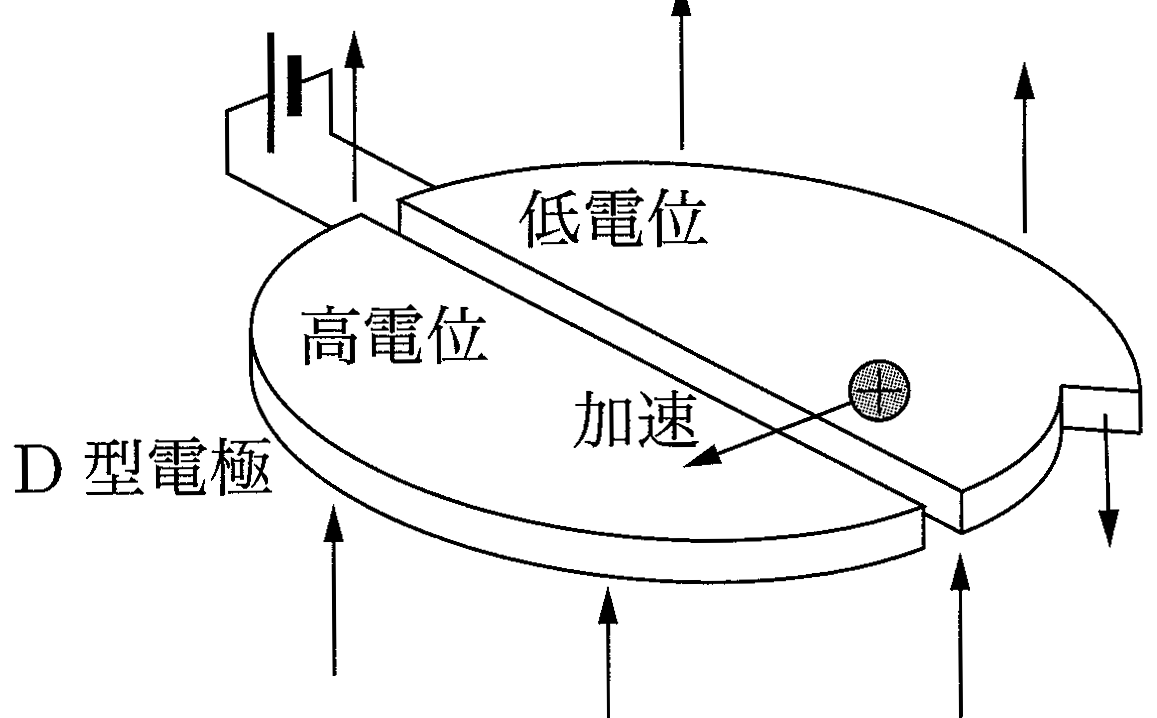
\includegraphics[keepaspectratio,width=52mm]{fig/n29_a98_zu2.png}\end{center}
電池のスイッチ切り替えでこれを行うのは面倒なので，交流電源を利用してDの電位を交互に反転させる．速さが大きいほど円運動の半径は大きくなるので，ギャップ通過で加速されるごとに円運動の半径は大きくなり，そのうち出口から出てくることになる．
\end{sisin}
\KaiHead
\begin{komon}
\ko{1} 荷電粒子が速さ$v$で半径$r$の円軌道を運動しているとき，中心方向の加速度の大きさは$\dfrac{v^2}{r}$となる．また，荷電粒子に作用している大きさ$qvB$のローレンツ力が向心力となっているので，この方向の運動方程式は$m\dfrac{v^2}{r}=qvB$．これを解いて，
       \[r=\frac{mv}{qB}\U{m}\Ans\]
\ko{2} 円運動の周期は，
       \[T=\frac{2\pi r}{v}=\frac{2\pi m}{qB}\U{s}\Ans\]
\ko{3} 等しく\Ans
\ko{4} この粒子を加速させるためには，サイクロトロンの電圧の周期とこの粒子の回転の周期とを等しくしなければならない．ゆえに，$\dfrac{1}{f_0}=\dfrac{2\pi M}{QB_0}$が満たされていなければならない．これを解いて，
       \[B_0=\frac{2\pi Mf_0}{Q}\U{Wb/m^2}\Ans\]
\ko{5} サイクロトロンから出てくる荷電粒子は，最大軌道半径$R$のところに達して円運動を行う粒子である．よって，この粒子がサイクロトロンを出てくる速さを$v_0$とすると，粒子の円運動の回転数が$f_0\U{Hz}$であることに注意して，$v_0=(2\pi f_0)\cdot R$．よって出てくる粒子のエネルギー$E$（粒子の運動エネルギー）は，
       \[E=\frac{1}{2}Mv_0^2=2\pi^2f_0^2MR^2\U{J}\Ans\]
\end{komon}
\begin{bsHosoku}{参考}
サイクロトロンのキーポイントとなっているのは，{\gtfamily 磁場中を等速円運動する荷電粒子の周期が半径および速さによらない}ということである．この性質のため，D型電極の電位の正負反転の周期が一定となり，一定周波数の交流電圧をかければよいことになるのである．
\end{bsHosoku}

\end{multicols}
